%Fred, Yuhan NSF REU Sites Aug 2021
\documentclass[11pt]{NSFamsart}
\usepackage{latexsym,amsfonts,amsmath,amssymb,amsthm,epsfig,extdash,multirow}
\usepackage{stackrel,tabularx,mathtools,longtable,xspace}  
\usepackage[shortlabels]{enumitem}
\usepackage[dvipsnames]{xcolor}
\usepackage[numbers,sort&compress]{natbib}
\usepackage{accents, booktabs}
\usepackage[hyphens]{url}
\usepackage[breaklinks]{hyperref}
\usepackage{algorithm, algorithmicx}
\usepackage{anyfontsize, microtype}
\usepackage{cleveref}
\usepackage{wrapfig}
\usepackage[font=small,labelfont=bf]{caption}
\usepackage{bm}
\usepackage{wrapfig}
\usepackage[normalem]{ulem}

\usepackage{algpseudocode}
\algnewcommand\algorithmicparam{\textbf{Parameters:}}
\algnewcommand\PARAM{\item[\algorithmicparam]}
\algnewcommand\algorithmicinput{\textbf{Input:}}
\algnewcommand\INPUT{\item[\algorithmicinput]}
\algnewcommand\RETURN{\State \textbf{Return }}
\DeclareMathOperator{\ALG}{ALG}

%%%%%%%%%%%%%%% Margins and Page Numbers %%%%%%%%%%%%%%%%%%%%%%%%%%%%%% 
\voffset 0.23in  %Made to satisfy Research.gov compliance
\hoffset 0.02in
\textheight 8.91in
\textwidth 6.44in
\setlength{\oddsidemargin}{0in}
\setlength{\evensidemargin}{0in}
%\thispagestyle{empty} \pagestyle{empty} %to eliminate page numbers for upload
\thispagestyle{plain} \pagestyle{plain} %to add back page numbers
%%%%%% Squeeze the space %%%%%%%%%%%%%%%%%%%%%%%%%%%%%% 
%\renewcommand{\baselinestretch}{0.97}
%%%%%%Squeeze the space %%%%%%%%%%%%%%%%%%%%%%%%%%%%%% 
%%%%%%%%%%%%%%% Margins and Page Numbers %%%%%%%%%%%%%%%%%%%%%%%%%%%%%% 


\headsep-0.6in


%%% Ideas


%\usepackage{showlabels}
\newcommand{\Upara}[1]{\noindent\underline{\upshape #1}:}

\newcommand{\myshade}{60}
\colorlet{mylinkcolor}{violet}
\colorlet{mycitecolor}{violet}
%\colorlet{mycitecolor}{OliveGreen}
\colorlet{myurlcolor}{YellowOrange}

\hypersetup{
	linkcolor  = mylinkcolor!\myshade!black,
	citecolor  = mycitecolor!\myshade!black,
	urlcolor  = myurlcolor!\myshade!black,
	colorlinks = true,
}


% This package prints the labels in the margin
%\usepackage[notref,notcite]{showkeys}



\newcommand{\FH}{\hyperlink{FHlink}{FH}\xspace}
\newcommand{\MH}{\hyperlink{MHlink}{MH}\xspace}
\newcommand{\GP}{\hyperlink{GPlink}{GP}\xspace}
\newcommand{\SM}{\hyperlink{SMlink}{SM}\xspace}
\newcommand{\SCTC}{\hyperlink{SCTClink}{SCC}\xspace}
\newcommand{\AO}{\hyperlink{AOlink}{AO}\xspace}
\newcommand{\MM}{\hyperlink{MMlink}{MM}\xspace}
\newcommand{\TS}{\hyperlink{TSlink}{TS}\xspace}
\newcommand{\GEF}{\hyperlink{GEFlink}{GEF}\xspace}
\newcommand{\YD}{\hyperlink{YDlink}{YD}\xspace}
\newcommand{\JR}{\hyperlink{JRlink}{JR}\xspace}
\newcommand{\LlAJR}{\hyperlink{LlAJRlink}{LlAJR}\xspace}
\newcommand{\LJ}{\hyperlink{LJlink}{LJ}\xspace}
\newcommand{\XT}{\hyperlink{XTlink}{XT}\xspace}
\newcommand{\KZ}{\hyperlink{KZlink}{KZ}\xspace}
\newcommand{\DL}{\hyperlink{DLlink}{DL}\xspace}
\newcommand{\XZ}{\hyperlink{XZlink}{XZ}\xspace}
\newcommand{\JL}{\hyperlink{JLlink}{JL}\xspace}
\newcommand{\YZ}{\hyperlink{YZlink}{YZ}\xspace}
\newcommand{\AS}{\hyperlink{ASlink}{AS}\xspace}
\newcommand{\CLT}{\hyperlink{CLTlink}{CLT}\xspace}
\newcommand{\PN}{\hyperlink{PNlink}{PN}\xspace}
\newcommand{\LK}{\hyperlink{LKlink}{LK}\xspace}
\newcommand{\SL}{\hyperlink{SLlink}{SL}\xspace}
\newcommand{\QOIs}{\hyperlink{QOIlink}{QOIs}\xspace}
\newcommand{\POIs}{\hyperlink{POIlink}{POIs}\xspace}
\newcommand{\MAA}{\hyperlink{MAAlink}{MAA}\xspace}
\newcommand{\JMM}{\hyperlink{JMMlink}{JMM}\xspace}
\newcommand{\SIAM}{\hyperlink{SIAMlink}{SIAM}\xspace}
\newcommand{\AWM}{\hyperlink{AWMlink}{AWM}\xspace}
\newcommand{\NAM}{\hyperlink{NAMlink}{NAM}\xspace}
\DeclareMathOperator{\QOI}{QOI} %Quantity of Interest
\DeclareMathOperator{\POI}{POI} %Parameter of Interest
\newcommand{\MSIs}{\hyperlink{MSIlink}{MSIs}\xspace}

%%list of acronyms with links
\newcommand{\QMCSoft}{QMCSoft\xspace}
\newcommand{\GAIL}{GAIL\xspace}
\newcommand{\QMC}{QMC\xspace}
\newcommand{\IIDMC}{IID MC\xspace}
\newcommand{\SAMSIQMC}{SAMSI-QMC\xspace}
\newcommand{\SciPy}{SciPy\xspace}
\newcommand{\GSL}{GSL\xspace}
\newcommand{\NAG}{NAG\xspace}
\newcommand{\MATLAB}{MATLAB\xspace}
\newcommand{\Chebfun}{Chebfun\xspace}
\newcommand{\Rlang}{R\xspace}
\newcommand{\Julia}{Julia\xspace}


\newtheorem{theorem}{theorem}


\providecommand{\FHickernell}{Hickernell}
\newcommand{\hf}{\widehat{f}}
\newcommand{\hg}{\widehat{g}}
\newcommand{\hI}{\hat{I}}
\newcommand{\hatf}{\hat{f}}
\newcommand{\hatg}{\hat{g}}
\newcommand{\tf}{\widetilde{f}}
\newcommand{\tbf}{\tilde{\bff}}
%\DeclareMathOperator{\Pr}{\mathbb{P}}
\newcommand{\eff}{\textup{eff}}

% Math operators
\DeclareMathOperator{\cost}{COST}
\DeclareMathOperator{\comp}{COMP}
\DeclareMathOperator{\loss}{loss}
\DeclareMathOperator{\lof}{lof}
\DeclareMathOperator{\reg}{reg}
\DeclareMathOperator{\CV}{CV}
\DeclareMathOperator{\size}{wd}
%\DeclareMathOperator{\GP}{\mathcal{G} \! \mathcal{P}}
\DeclareMathOperator{\erf}{erf}
\DeclareMathOperator*{\argmax}{arg\,max}
\DeclareMathOperator*{\argmin}{arg\,min}
\DeclareMathOperator{\Ans}{ANS}
\DeclareMathOperator{\Var}{Var}
\DeclareMathOperator{\APP}{\widehat{\QOI}}
\DeclareMathOperator{\SURR}{SM} %surrogate model
\DeclareMathOperator{\STREND}{ST} %surrogate trend
\DeclareMathOperator{\SVAR}{SV} %surrogate variation
\DeclareMathOperator{\SVARERR}{SVU} %surrogate variation uncertainty
\newcommand{\MLS}{\textrm{MLS}\xspace} %distance weighted least squares, also known as moving least squares
%\DeclareMathOperator{\ALG}{ALG}
\DeclareMathOperator{\ERR}{ERR}
\DeclareMathOperator{\VAL}{ACQ}
\DeclareMathOperator{\OPER}{OPER}
\DeclareMathOperator{\INT}{INT}
\DeclareMathOperator{\MIN}{MIN}
\DeclareMathOperator{\ID}{ID}
\DeclareMathOperator{\APPMIN}{\widehat{\MIN}}
\DeclareMathOperator{\APPID}{\widehat{\ID}}
\DeclareMathOperator{\MINVAL}{MINACQ}
\DeclareMathOperator{\IDVAL}{IDACQ}
\DeclareMathOperator{\SURRERR}{SU}
\DeclareMathOperator{\MINERR}{MERR}
\DeclareMathOperator{\IDERR}{IDERR}
\DeclareMathOperator{\Prob}{\mathbb{P}}
\DeclareMathOperator{\diag}{diag}
\DeclareMathOperator{\dist}{dist}
\DeclareMathOperator{\filldis}{fill}
\DeclareMathOperator{\sep}{sep}
\DeclareMathOperator{\avg}{avg}
\DeclareMathOperator{\vol}{vol}
\DeclareMathOperator{\cov}{cov}
\DeclareMathOperator{\std}{std}
\DeclareMathOperator{\var}{var}
\newcommand{\TREND}{\textup{T}}
\newcommand{\VAR}{\textup{V}}
\newcommand{\LS}{\textup{MLS}}







\newcommand{\reals}{{\mathbb{R}}}
\newcommand{\naturals}{{\mathbb{N}}}
\newcommand{\natzero}{{\mathbb{N}_0}}
\newcommand{\integers}{{\mathbb{Z}}}
\newcommand\expect{{\mathbb{E}}}
\def\il{\left \langle}
\def\ir{\right \rangle}
\def\e{\varepsilon}
\def\g{\gamma}
\def\l{\lambda}
\def\b{\beta}
\def\a{\alpha}
\def\lall{\Lambda^{{\rm all}}}
\def\lstd{\Lambda^{{\rm std}}}

\newcommand{\vf}{\boldsymbol{f}}
\newcommand{\hV}{\widehat{V}}
\newcommand{\tV}{\widetilde{V}}
\newcommand{\fraku}{\mathfrak{u}}
\newcommand{\hcut}{\mathfrak{h}}
\newcommand{\tOmega}{\widetilde{\Omega}}
\newcommand{\tvarrho}{\widetilde{\varrho}}

\newcommand{\bbE}{\mathbb{E}}
\newcommand{\tQ}{\widetilde{Q}}
\newcommand{\mA}{\mathsf{A}}
\newcommand{\mB}{\mathsf{B}}
\newcommand{\mC}{\mathsf{C}}
\newcommand{\mD}{\mathsf{D}}
\newcommand{\mG}{\mathsf{G}}
\newcommand{\mH}{\mathsf{H}}
\newcommand{\mI}{\mathsf{I}}
\newcommand{\bbK}{\mathbb{K}}
\newcommand{\mK}{\mathsf{K}}
\newcommand{\tmK}{\widetilde{\mathsf{K}}}
\newcommand{\mL}{\mathsf{L}}
\newcommand{\mM}{\mathsf{M}}
\newcommand{\mP}{\mathsf{P}}
\newcommand{\mQ}{\mathsf{Q}}
\newcommand{\mR}{\mathsf{R}}
\newcommand{\mX}{\mathsf{X}}
\newcommand{\mPhi}{\mathsf{\Phi}}
\newcommand{\mPsi}{\mathsf{\Psi}}
\newcommand{\mLambda}{\mathsf{\Lambda}}
\newcommand{\cube}{[0,1]^d}
\newcommand{\design}{\{\bx_i\}_{i=1}^n}




\newcommand{\bone}{\boldsymbol{1}}
\newcommand{\bzero}{\boldsymbol{0}}
\newcommand{\binf}{\boldsymbol{\infty}}
\newcommand{\ba}{{\boldsymbol{a}}}
\newcommand{\bb}{{\boldsymbol{b}}}
\newcommand{\bc}{{\boldsymbol{c}}}
\newcommand{\bd}{{\boldsymbol{d}}}
\newcommand{\be}{{\boldsymbol{e}}}
\newcommand{\bff}{{\boldsymbol{f}}}
\newcommand{\bhh}{{\boldsymbol{h}}}
\newcommand{\beps}{{\boldsymbol{\varepsilon}}}
\newcommand{\tbeps}{\tilde{\beps}}
\newcommand{\bx}{{\boldsymbol{x}}}
\newcommand{\bX}{{\boldsymbol{X}}}
\newcommand{\bh}{{\boldsymbol{h}}}
\newcommand{\bj}{{\boldsymbol{j}}}
\newcommand{\bk}{{\boldsymbol{k}}}
\newcommand{\bg}{{\boldsymbol{g}}}
\newcommand{\bn}{{\boldsymbol{n}}}
\newcommand{\br}{{\boldsymbol{r}}}
\newcommand{\bv}{{\boldsymbol{v}}}
\newcommand{\bu}{{\boldsymbol{u}}}
\newcommand{\by}{{\boldsymbol{y}}}
\newcommand{\bt}{{\boldsymbol{t}}}
\newcommand{\bz}{{\boldsymbol{z}}}
\newcommand{\bvarphi}{{\boldsymbol{\varphi}}}
\newcommand{\bgamma}{{\boldsymbol{\gamma}}}
\newcommand{\bphi}{{\boldsymbol{\phi}}}
\newcommand{\bpsi}{{\boldsymbol{\psi}}}
\newcommand{\btheta}{{\boldsymbol{\theta}}}
\newcommand{\bnu}{{\boldsymbol{\nu}}}
\newcommand{\balpha}{{\boldsymbol{\alpha}}}
\newcommand{\bbeta}{{\boldsymbol{\beta}}}
\newcommand{\bo}{{\boldsymbol{\omega}}}  %GF added
\newcommand{\newton}[2]{\left(\begin{array}{c} #1\\ #2\end{array}\right)}
\newcommand{\anor}[2]{\| #1\|_{\mu_{#2}}}
\newcommand{\satop}[2]{\stackrel{\scriptstyle{#1}}{\scriptstyle{#2}}}
\newcommand{\setu}{{\mathfrak{u}}}

\newcommand{\me}{\textup{e}}
\newcommand{\mi}{\textup{i}}
\def\d{\textup{d}}
\def\dif{\textup{d}}
\newcommand{\cc}{\mathcal{C}}
\newcommand{\cb}{\mathcal{B}}
\newcommand{\ca}{\mathcal{A}}
\newcommand{\cl}{L}
\newcommand{\ct}{\mathcal{T}}
\newcommand{\cx}{{\Omega}}
\newcommand{\cala}{{\mathcal{A}}}
\newcommand{\calc}{{\mathcal{C}}}
\newcommand{\calf}{{\mathcal{F}}}
\newcommand{\calfd}{{\calf_d}}
\newcommand{\calh}{{\mathcal{H}}}
\newcommand{\tcalh}{{\widetilde{\calh}}}
\newcommand{\calI}{{\mathcal{I}}}
\newcommand{\calhk}{\calh_d(K)}
\newcommand{\calg}{{\mathcal{G}}}
\newcommand{\calgd}{{\calg_d}}
\newcommand{\caln}{{\mathcal{N}}}
\newcommand{\calp}{{\mathcal{P}}}
\newcommand{\cals}{{\mathcal{S}}}
\newcommand{\calu}{{\mathcal{U}}}
\newcommand{\cL}{\mathcal{L}}
\newcommand{\cP}{\mathcal{P}}
\newcommand{\cT}{\mathcal{T}}
\newcommand{\cK}{\mathcal{K}}
\newcommand{\fA}{\mathfrak{A}}
\newcommand{\fC}{\mathfrak{C}}
\newcommand{\fF}{\mathfrak{F}}
\newcommand{\fL}{\mathfrak{L}}
\newcommand{\fT}{\mathfrak{T}}
\newcommand{\fU}{\mathfrak{U}}
\newcommand{\hS}{\widehat{S}}

\def\abs#1{\ensuremath{\left \lvert #1 \right \rvert}}
\newcommand{\bigabs}[1]{\ensuremath{\bigl \lvert #1 \bigr \rvert}}
\newcommand{\norm}[2][{}]{\ensuremath{\left \lVert #2 \right \rVert}_{#1}}
\newcommand{\ip}[3][{}]{\ensuremath{\left \langle #2, #3 \right \rangle_{#1}}}
\newcommand{\bignorm}[2][{}]{\ensuremath{\bigl \lVert #2 \bigr \rVert}_{#1}}
\newcommand{\Bignorm}[2][{}]{\ensuremath{\Bigl \lVert #2 \Bigr \rVert}_{#1}}
\newcommand{\calm}{{\mathfrak{M}}}

\newcommand{\des}{\{\bx_i\}}
\newcommand{\desinf}{\{\bx_i\}_{i=1}^{\infty}}
\newcommand{\desn}{\{\bx_i\}_{i=1}^n}
\newcommand{\wts}{\{g_i\}_{i=1}^N}
\newcommand{\wtsn}{\{g_i\}_{i=1}^N}
\newcommand{\datan}{\{y_i\}_{i=1}^N}

%FJH added
\newcommand{\Order}{\mathcal{O}}
\newcommand{\ch}{\mathcal{H}}
\newcommand{\tch}{{\widetilde{\ch}}}
\newcommand{\veps}{\boldsymbol{\varepsilon}}
\DeclareMathOperator{\best}{best}
\newcommand{\hmu}{\hat{\mu}}
\newcommand{\hsigma}{\hat{\sigma}}
\newcommand{\tK}{\widetilde{K}}
%\newcommand{\Matlab}{{\sc Matlab}\xspace}
\newcommand{\abstol}{\varepsilon_{\text{a}}}
\newcommand{\reltol}{\varepsilon_{\text{r}}}

\newcommand\starred[1]{\accentset{\star}{#1}}

\newcommand{\designInf}{\{\bx_i\}_{i=1}^\infty}
\newcommand{\dataN}{\bigl\{\bigl(\bx_i,f(\bx_i)\bigr)\bigr\}_{i=1}^n}
\newcommand{\dataNp}{\bigl\{\bigl(\bx_i,f(\bx_i)\bigr)\bigr\}_{i=1}^{n'}}
\newcommand{\dataNo}{\bigl\{\bigl(\bx_i,f(\bx_i)\bigr)\bigr\}_{i=1}^{n_0}}
\newcommand{\ErrN}{\ERR\bigl(\dataN,n\bigr)}
\newcommand{\fint}{f_{\text{int}}}
\newcommand{\inflate}{\fC}
\newcommand{\Ex}{\mathbb{E}}
\newcommand{\IIDSim}{\overset{\text{IID}}{\sim}}
 
\newcommand\KL{\mathrm{KL}}
\newcommand\x{\bm{x}}
\newcommand\dd{\mathrm{d}}

\definecolor{MATLABOrange}{rgb}{0.85,  0.325, 0.098}


%\setcounter{page}{1}


\setlist[description]{font=\normalfont\itshape, labelindent = 0.5cm}
\setlist[itemize]{leftmargin=5ex}

\makeatletter
\newenvironment{varsubequations}[1]
 {%
  \addtocounter{equation}{-1}%
  \begin{subequations}
  \renewcommand{\theparentequation}{#1}%
  \def\@currentlabel{#1}%
 }
 {%
  \end{subequations}\ignorespacesafterend
 }
\makeatother


\newcommand{\FJHNote}[1]{{\color{blue}Fred: #1}}
\newcommand{\YDNote}[1]{{\color{magenta}Yuhan: #1}}
\newcommand{\scnote}[1]{{\color{green}SC: #1}}
\newcommand{\LKnote}[1]{{\color{brown}LKl
: #1}}

% Notes on the paper for communicating with coauthors
\newif\ifnotesw \noteswtrue
\newcommand{\notes}[1]{\ifnotesw \textcolor{red}{  $\clubsuit$\ {\sf \bf \it  #1}\ $\clubsuit$  }\fi}
%\noteswfalse   % comment this line out to turn on style notes 


\begin{document}
%\setlength{\leftmargini}{2.5ex}

\iffalse
More definite words than "hope", like "will"
SURE program -> SURE
SC: REU I nixed it
The Office of ...
Office of Research Integrity and Compliance
Open scholarship
computational(?) data science or computation and data science

\fi

\begin{center}
\Large 
\textbf{REU Site: Summer Undergraduate Research Experience (SURE) at Illinois Tech}
\end{center}


%  \setcounter{tocdepth}{1}
%  \tableofcontents
%  \vspace{-10ex}

\section{Overview} 
SURE will engage undergraduate students---\emph{especially those from underrepresented groups and academic institutions where research opportunities are limited}---in innovative computational mathematics and machine learning research.  SURE students will  be embedded in existing, active research groups. They will acquire both ``hard'' academic and ``soft'' communication and teamwork skills.  SURE students will be prepared and inspired to pursue graduate study in mathematics, statistics, or a related field in preparation for research careers in academia or industry.

SURE will involve \emph{ten undergraduate students (divided into three groups), three faculty mentors, and three graduate students} each summer for three years at the Illinois Institute of Technology (Illinois Tech). At least one faculty mentor and one graduate student will come from the underrepresented group. SURE participants will engage in a \emph{ten-week program from May to July}, working in groups of three or four under faculty mentors' supervision and with graduate students' assistance. Faculty mentors will continue to advise SURE participants during the following academic year to write up their results for publication and to support them as they transition into graduate schools. In addition, SURE will provide financial support for students to present their research results at professional conferences and workshops.
SURE will be prepared to go virtual or hybrid if public health conditions require so.

The SURE experience will put the Illinois Tech Department of Applied Mathematics in a better position to recruit and mentor undergraduate researchers---especially those from underrepresented minorities---after SURE funding ends. SURE funding will help us build relationships with feeder institutions, who will continue to send us their students.  Our department will continue to use the mentoring programs and associated materials developed in SURE long term.  Sharing the organization and implementation of these programs across research groups will lighten the load on any particular group. We will establish a culture among our graduate and undergraduate students that those who are a few steps ahead mentor those behind them.

The acronym SURE plays a dual role in highlighting our objectives.


\begin{figure}[bh]
    \centering
    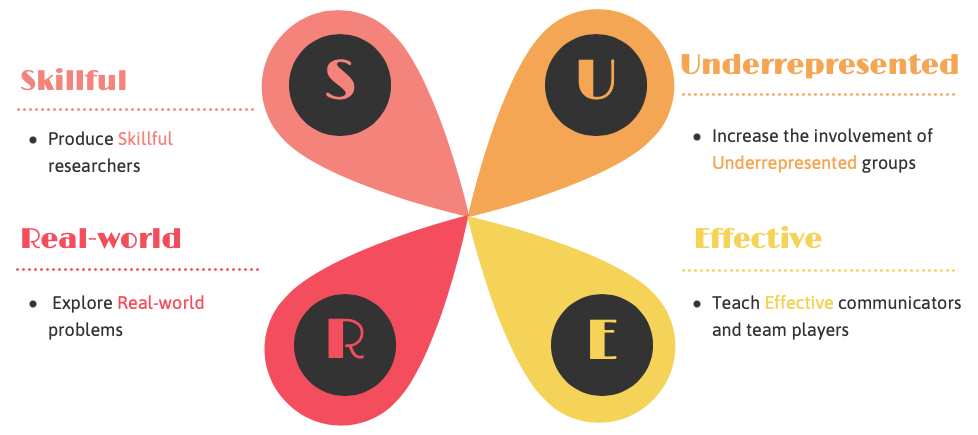
\includegraphics[width = 14cm]{SURE_1_3.png}
    \caption{Objectives of {\bf S}ummer {\bf U}ndergraduate {\bf R}esearch {\bf E}xperience Program}
    \label{fig:sure_obj}
\end{figure}

SURE students will be trained as \uppercase{\textbf{skillful}} researchers with essential computational and data skills. 
We will prioritize recruiting \uppercase{\textbf{underrepresented}} students, including women, underrepresented racial minorities, and students with disabilities. 
SURE students will explore 
\uppercase{\textbf{Real-world}} research problems and learn to pose questions, collect preliminary findings, modify their questions as necessary, and pursue answers. 
SURE students will learn to 
be \uppercase{\textbf{effective}} in communication, teamwork,  professionalism, and responsibility. 
With the support of our Illinois Tech family and other community members, we are dedicated to achieving these objectives via the plans and means described in this proposal. 



%\begin{itemize}



%\item SURE students will be trained as \uppercase{\textbf{skillful}} researchers with important computational and data skills.  This will be done not only through their research projects but also through tutorials and workshops tailored to fill the gaps in their preparation and help them understand the cutting edge of the problems that they are tackling.  Graduate students and faculty will engage in individual mentoring. The skills they learn will prepare them to be successful researchers at the PhD level. 


%\item SURE will heavily recruit \uppercase{\textbf{underrepresented}} students, including women, underrepresented racial minorities, and students with disabilities.  A few such students may come from Illinois Tech, but others will come from the minority-serving institutions (MSIs) in Chicagoland or elsewhere with personal reasons for spending the summer in Chicago.  
%\item SURE students will explore \uppercase{\textbf{Real-world}} research problems. They will learn to pose questions, collect preliminary findings, modify their questions as necessary, and pursue answers.  Mentors will help them think through why a question might be important or interesting and what steps might be taken to answer it.  However, the SURE students will be allowed to explore questions for which we cannot be assured of their success in finding the answer. \scnote{Change ``be assured'' to ``assure''?}

%\item SURE students will learn to be \uppercase{\textbf{effective}} in communication, teamwork,  professionalism, and responsibility.  SURE students will learn to communicate what they are doing to various audiences: their team members, mathematicians unfamiliar with their work, and their friends and family who are not mathematically literate.  They will learn to work with team members who may have culturally different ways of working or communicating.  Presentations by Illinois Tech experts in responsible conduct of research, Title IX, and diversity, equity, and inclusion will strengthen their ethical foundation.
%\end{itemize}


%\subsection{Targeted Student Participants}\label{sec:targetstd}
The targeted student participants will primarily be rising third or fourth-year undergraduates with a  background
in mathematics and statistics, including at least univariate calculus and programming.  Priority will be given to students 
\begin{itemize}
\item From \hypertarget{MSIlink} Minority Serving Institutions (\MSIs),
\item From institutions with limited research opportunities will be given high priority
\item Veterans of the US armed services,  and 
\item First-generation college students 
\end{itemize}
To recruit these targeted students,  we have several external collaborators who will help us recruit students and promote SURE at their institutions: Morgan State University (MSU), a public historically black college and university (HBCU), Chicago State University (CSU), the only PBI (Predominantly Black Serving Institution) in the Midwest, Northeastern Illinois University (NEIU), a Hispanic-Serving Institution (HSI), and Wheaton College, a liberal arts college with limited research opportunities. 



\iffalse Yuhan: It is hard to reach the minorities goal

We will admit our undergraduates according to the following profile: 
\begin{enumerate}[1)]
 \item \emph{At least 60\%} from underrepresented groups including women, racial minorities, and persons with disabilities;
 \item \emph{At least 30\%} underrepresented racial minorities;
 \item \emph{At least half} from academic institutions where research opportunities are limited
(including two-year colleges), and 
\item \emph{At least 60\%} from outside Illinois Tech.
\end{enumerate}

\fi

%\subsection{Intellectual Focus}
The program will engage SURE
participants in the model development, algorithm design, data sampling, analysis, and implementation
of mathematical, statistical, and computational methods, mainly as they apply to specific problems
in the real world.  SAS Institute Inc, one of the collaborators, will provide at least one project for SURE and corresponding supervisors to guide students on the company side. \FJHNote{How about Intel/SigOpt?}All proposed research projects in this program are mainly designed to stimulate
the research interests of SURE participants in applied mathematics, statistics, data science, and computational
methods to fundamental problems in the real world and to inspire them to pursue graduate education. This
program aims to achieve a long-term positive impact on their career decisions to pursue academic and
professional careers in STEM disciplines.



 

%On Day 1, the research projects will be presented to SURE participants along with physical and biological background and an overview of some of the mathematical, statistical, or computational techniques involved in the project. Weeks 1-2 of the program will be devoted to tutorials/workshops/courses given by faculty mentors/graduate students to provide the participants with the necessary technical tools including some short courses, open scholarship,  computer skills, and background introduction to begin the projects. By the end of Week 2, students will have decided on a research project with the assistance of their assigned faculty mentor during the admission and present the initial problems they work with on Week 3 and midterm progress on Week 6 or 7. During Week 9, students will begin writing their conclusions and preparing a poster presentation. In Week 10, students will finalize their reports and poster presentations. SURE Poster Day will be held on the last morning, where each student or group of students describes their problem and explains their main findings to other students and faculty viewing their poster.




\section{Nature of Student Activities}
\subsection{SURE Program Schedule}
\label{sec:SURESchedule}
Each SURE student will be
assigned a mentor and research area based on their preference during admission. SURE students and faculty
mentors will communicate in real-time through Slack or a similar platform. There will be weekly SURE group meetings, as described below.  In addition, each
faculty mentor will discuss their ongoing projects with their SURE students to explain the broader context of their research. SURE students will be encouraged to attend regular research group seminars (generally biweekly) to learn state-of-the-art research topics and interact
with the invited speakers. Three graduate students selected from the Ph.D. students
of the faculty mentors will assist SURE participants. They will
directly assist students with mathematics and statistics-related
concepts, discuss the projects and offer suggestions. The Applied Math department will provide SURE participants with
a shared office populated by graduate students, which
allows more significant interaction between the two groups. 
PIs will organize social activities to provide recreation
and build team-cooperation relationships for all involved participants: (1) Orientation luncheon; (2) Weekly SURE group Math Tea time; (3) BBQ
cookout; (4) Baseball games;  (5)
 Final presentation reception.



\centerline{\emph{Week 1: Project Selection and Short Courses/Tutorials/Workshops}}
%\vspace{-2ex}
\begin{figure}[h]
    \centering
    {\footnotesize \textsf{
    \begin{tabular}{c>{\centering}p{23ex}>{\centering}p{20ex}>{\centering}p{12ex}>{\centering}p{12ex}>{\centering}p{15ex}}
         Week 1 &  Day 1 & Day 2 & Day 3 & Day 4 & Day 5 \tabularnewline \toprule
         Morning & Icebreaker Games \newline Projects Introduction 
         & Software Tutorial \newline Practice Projects 
         & Short Courses
         & Short Courses
         & Group Meeting with Mentor \tabularnewline \midrule
         Evening & Workshop on Research Integrity and Title IX
         & Git/LaTeX Tutorial \newline Practice Projects 
         & HW and \newline Q\&A
         & HW and \newline Q\&A \newline
         & Project Selection
    \end{tabular} }} \vspace{-3ex}
%    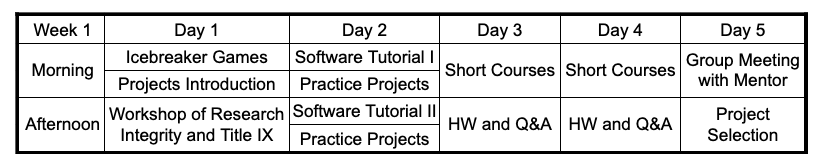
\includegraphics[width = 14cm]{FirstWeekSchedule.png}
    \caption{Schedule of the first week}
    \label{fig:1stweekschedule}
\end{figure}

\emph{Day 1} is orientation. All participants, faculty mentors, and three graduate students will introduce themselves in the morning and play icebreaker games. Afterward, mentors will present several sample project topics to students.
Participants will tour the Illinois Tech campus and facilities after lunch. In the afternoon, Illinois Tech staff will give workshops on research integrity, authorship, and Title IX.

\emph{Day 2} features the tutorials.
 We will offer software tutorials in the morning. PIs will choose the programming language based on needs of their projects and the participants. All participants will do a sample programming practice afterward. The afternoon tutorial will focus on technical writing, open scholarship, and reproducible research. Hands-on exercises will follow.
 
 \emph{Days 3 and 4} will offer several short courses that support the projects, such as linear algebra, probability, and statistics. The students will complete assignments to ensure they understand the concepts and how to use them.

 
Faculty mentors, graduate students, and Illinois staff experts will deliver these courses, tutorials, and workshops during the first four days.

\emph{Day 5}, SURE participants will meet their mentors in the morning to decide the projects to work on and discuss the plan in the following weeks. Mentors will provide the background
reading material and practice with computer software to initiate their projects. In the afternoon, each group will present their project selection and explain their plan for the next couple of weeks.


\centerline{\emph{Weeks 2-8: Research}}

SURE participants will pursue their projects. All participants will be encouraged to write blogs \cite{Hig21a} during the program. The blogs will help them learn to articulate their research problem and their findings to a more general audience. Faculty mentors and graduate
students will meet with SURE students weekly. During the regular meetings, faculty mentors and graduate students will communicate with SURE students and check on student progress. Faculty mentors will also hold regular office hours throughout the week to be available when students have questions.

\emph{Each Friday}, there will be a meeting of all SURE participants. The mornings of Weeks 2 through 4 will focus on helping students adapt to the program and become familiar with research. Tips and research experiences will shared by the SURE alumni and faculty. The mornings of Weeks 6 through 8 will focus on application to graduate programs and strategies for successful academic careers with presentations and exercises organized by the PIs. The morning presentations will  be concluded by a Math Tea.  In the afternoon each research group will give a 20-30 minute presentation reporting on their progress and challenges encountered. Faculty mentors and graduate students will provide suggestions and comments on the research and presentation.

\emph{In the morning of the Friday of Week 5,}
each group of students will make a 50-minute midterm presentation to all to show the progress made so far, challenges encountered, plans for the next few weeks, and help needed. Faculty mentors,
graduate students, and peers will give feedback and guidance. In the afternoon, there will be a BBQ cookout. During the BBQ time, all the participants, faculty mentors, and graduate students will have games together. A baseball game night  
will follow. All students and faculty will watch the White Sox game at the Guaranteed Rate Field, which is a short walk away.


\centerline{\emph{Weeks 9-10: Article, Slide Deck, and Poster Preparation}} 

SURE students will start preparing articles in Week 9. These may be drafts of submissions to undergraduate journals or portions of more substantial papers to refereed conference proceedings or regular academic journals. Students will also develop their slide decks from the midterm presentations into presentations suitable for a conference talk. We want students to understand how to communicate their work in different forums.  Articles, slide decks, and posters all have different requirements in terms of detail, word density, and layout. In addition, they will prepare posters for a final presentation at the end of the Week 10.  These articles, slide decks, and posters will be finalized in Week 10. The final poster presentation will be publicized through various campus channels. Each group will also give a final oral presentation followed.  The program for the day will end with each student receiving a certificate of participation from SURE. \FJHNote{Did I describe this correctly?}


\FJHNote{Fred stopped here.}

\subsection{Sample Projects }
Faculty mentors have designed projects with several possible levels of completion to ensure that SURE participants
make independent research contributions, gain valuable research experience, and enjoy a feeling of
accomplishment after achieving their research objectives. Project topics vary from theoretical study to applications in various fields, such as finance, physics, biology, etc. Five sample research projects are described as follows.
\YDNote{Add students' requirement and learning objectives in the sample project}
%\subsubsection{Pattern Forming Problems in Physical and Biological Systems}
Once the machine learning algorithms aforementioned are fully developed, we will implement them in real physical or biological problems, in particular, pattern formation in non-equilibrium dynamical systems.  From
a mathematical point of view, studies of the pattern formation can be
formulated as moving boundary problems with interfaces separating
different physical  domains.  In the last few decades, theories,
experiments, and nonlinear simulations have contributed to gain a
better understanding of the mechanisms ruling the pattern selection,
in which interfacial instability is the central question. 

Interfacial instabilities occur when driving forces compete with resistive forces and typically result in the formation of complex patterns. Examples can be found in a wide
variety of systems, including filamentary microorganisms \cite{alain},
growing biofilms \cite{dockery01,Mattei2018}, tumor growth  \cite{MJ2020,Kara2018}, silica tubes forming in electrically-driven metal salt solutions \cite{steinbock03,steinbock16}, smoldering flame fronts
\cite{zik98,Kagan2008}, or lava flows \cite{balmforth00, griffiths00,Roman2021} in which
the interface itself is defined by a reaction or a solidification, and
driven by the expanding growth of the interior. Resistive forces include surface tension, viscous dissipation, bending, elasticity, and viscoelasticity.

There are a few critical parameters (e.g., flow field and initial interface configuration) that can  be estimated via machine-learning (ML) methods. These parameters may be spatial and temporal dependent and their values will be an output from ML algorithms. We formulate this estimation as a Constrained Multi-Output Learning problem as follows: suppose there are $T$ outputs, $y_1, \ldots, y_T$, and these outputs are related by a set of  $P$ equations, which link the available experimental data and simulation results: $\Gamma_p(y_1, \ldots, y_T)=0, p=1, \ldots, P$. For example, these equations will arise from matching the time evolution of interface sizes and shapes from simulation predictions with experimental measurements, which will be obtained by post-processing the images and videos of the  dynamical process. We aim to learn the $T$ outputs jointly (instead of separately) while satisfying the $P$ constraints. 

\begin{wrapfigure}{r}{0.66\textwidth}
%  \centering
  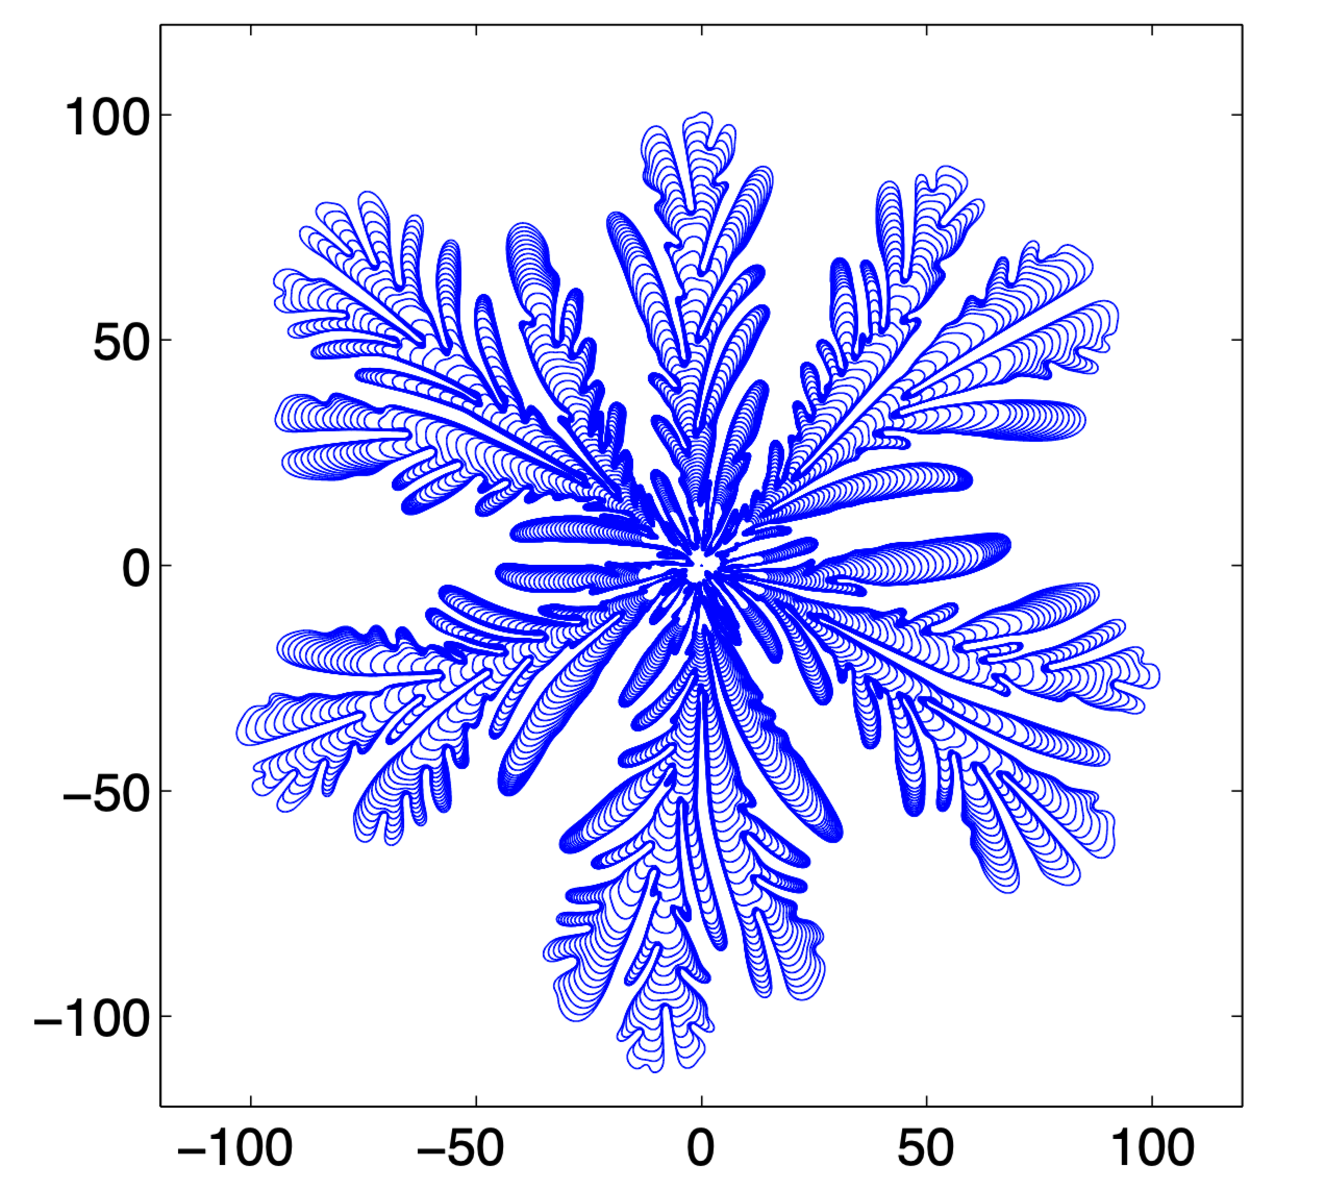
\includegraphics[scale=0.2]{Unstable}[a]
  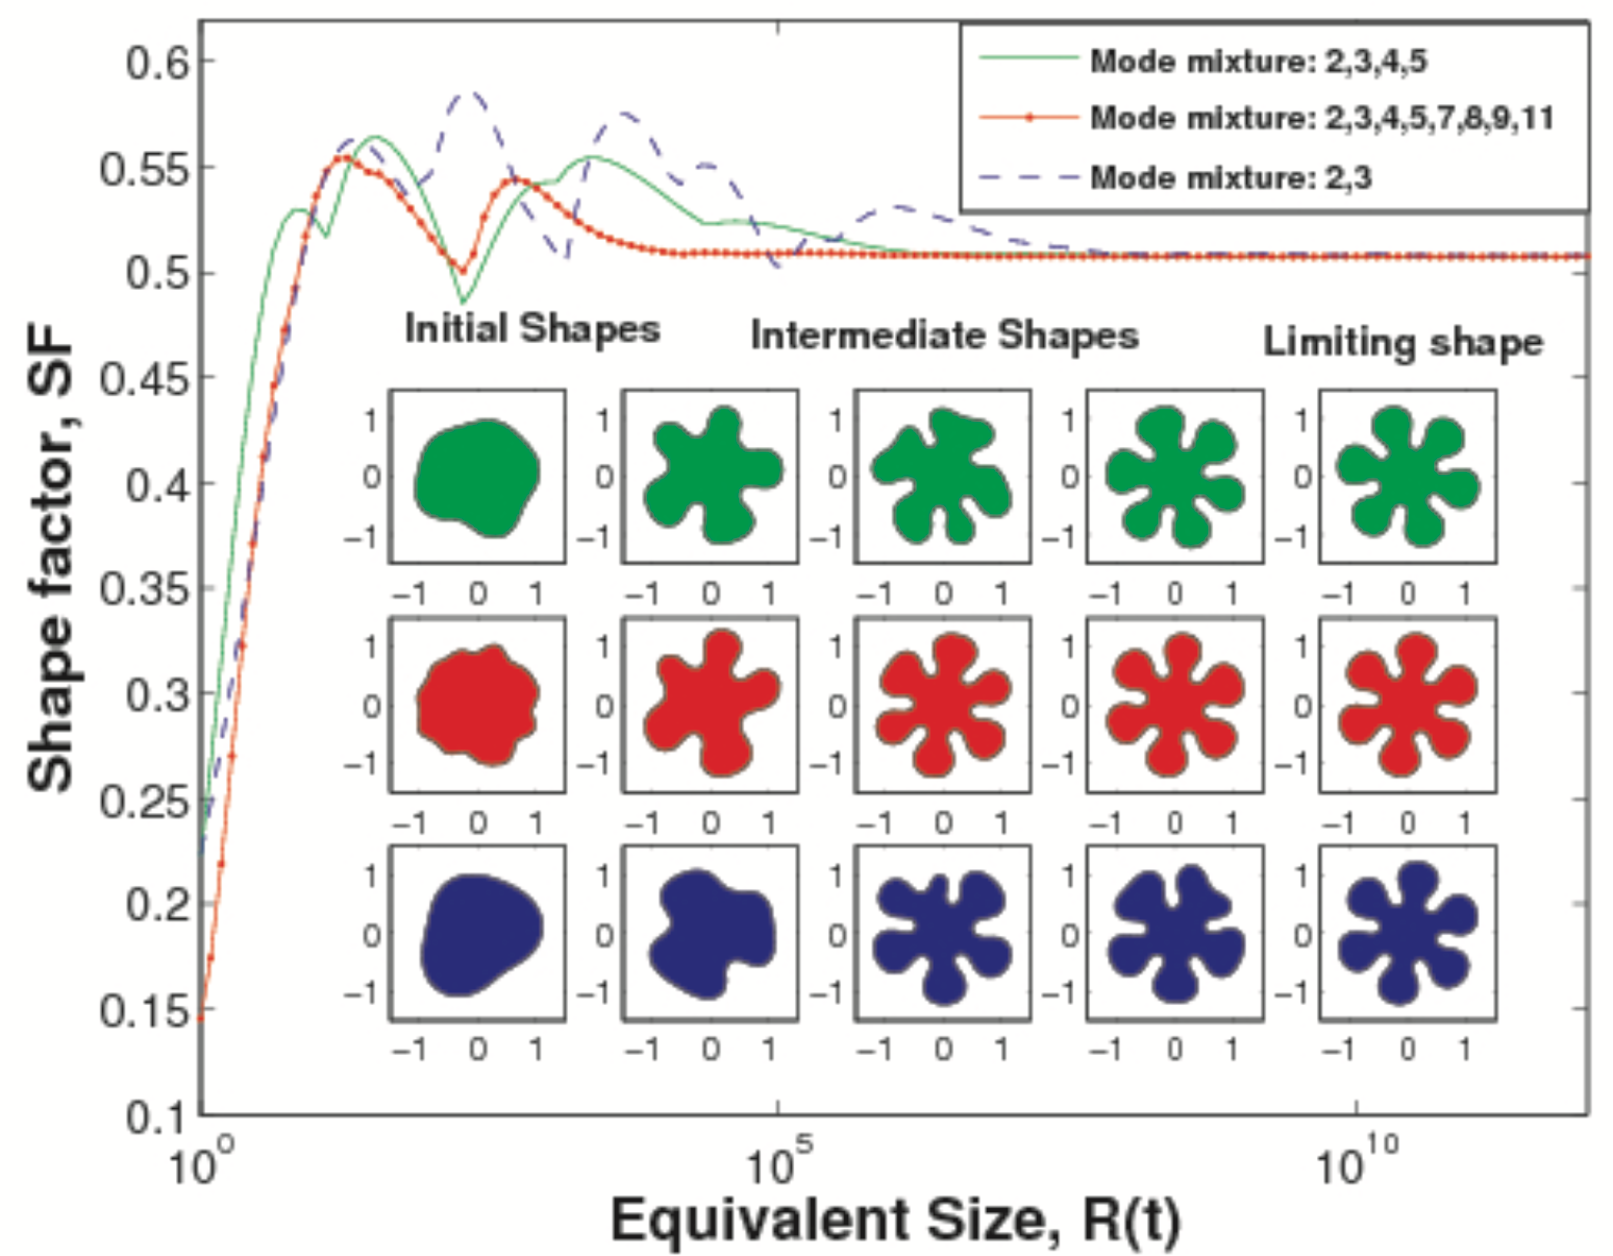
\includegraphics[scale=0.2]{Stable2}[b]
  \caption{An illustration of [a] unstable growth; [b] stable  dynamical equilibrium patterns with six-fold symmetry in a Hele-Shaw flow.}
  \label{figA}
  \end{wrapfigure}

 We propose a focused, coherent study of interfacial instabilities with an integrated analytical and numerical effort between faculty mentors' research groups. One sample project could be investigating a classic pattern forming system in fluid dynamics: viscous fingering in a Hele-Shaw cell \cite{saffman1986}. Our main goals are to investigate the nonlinear dynamics of interfaces and identify critical physical parameters (e.g., critical evolution time or size that an interface starts to equilibrate) via a ML approach such that a dynamical equilibrium state with certain symmetry can be achieved at a prescribed time or size. See Fig.~(\ref{figA})[a] for an illustration of unstable pattern development by repeated tip splitting process and Fig.~(\ref{figA})[b] for a six-fold self-similarly evolving pattern at dynamical equilibrium \cite{Li2009}. If time permits, we also plan to extend our research to avascular tumor growth using solvers recently developed in Li's group \cite{MJ2020}. The tumor problem involves more physical and biological parameters governing the dynamics and nutrient fields in tumor and  host tissues. We expect the developed machine learning algorithms to be more explorative of parameter space and to determine optimal parameter ranges for controlling the tumor-host interface.




%\begin{figure}[th!]
%  \centering
%  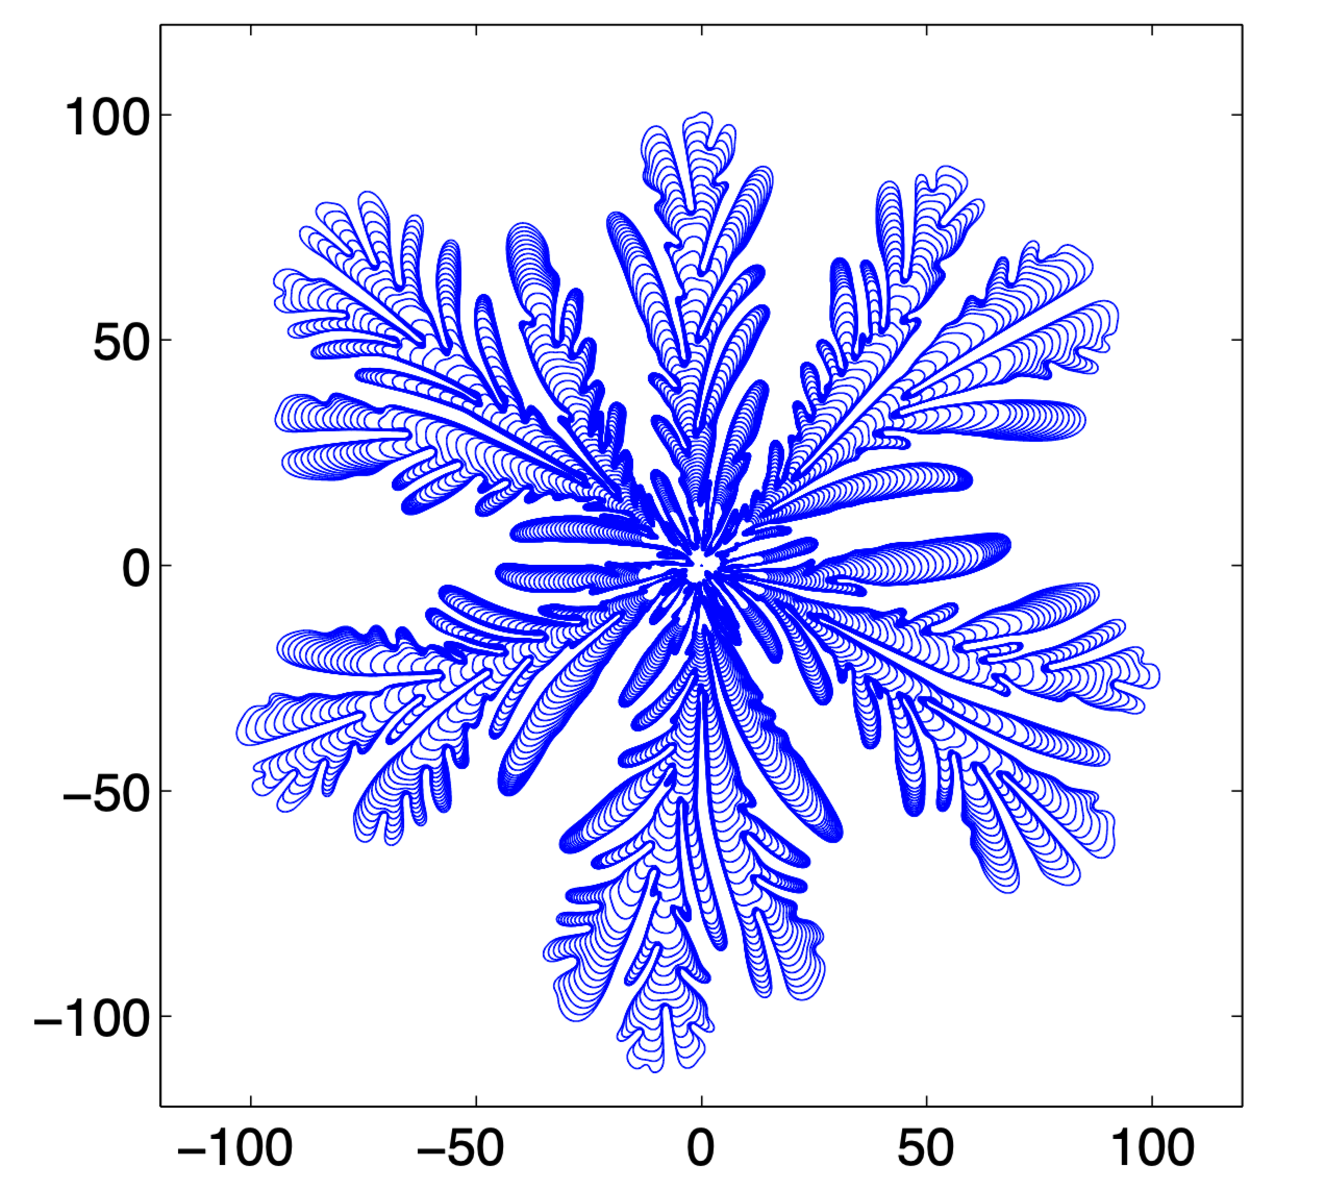
\includegraphics[scale=0.225]{Unstable}[a]
%  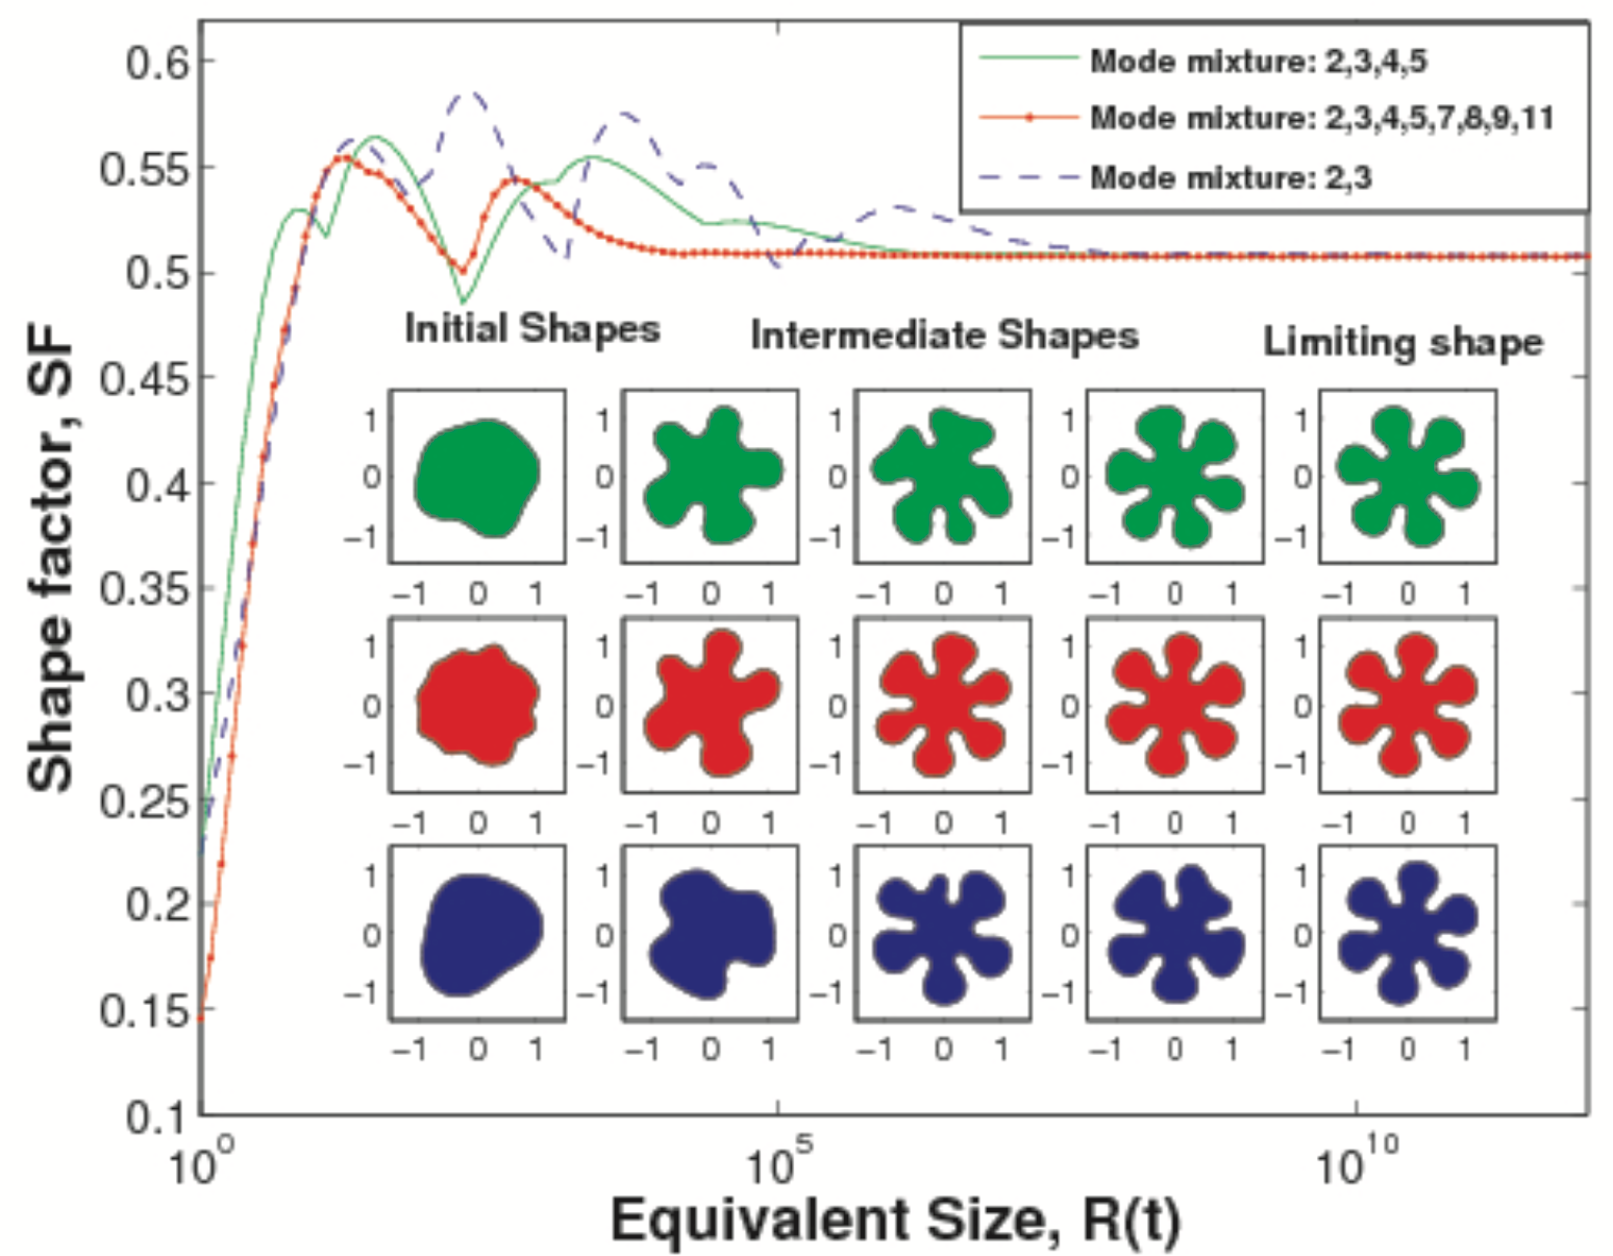
\includegraphics[scale=0.2]{Stable2}[b]
%  \caption{An illustration of unstable growth [a] and stable [b] dynamical patterns with six-fold symmetry in a Hele-Shaw flow.}
%  \label{figA}
%  \end{figure}


  


%There are many potential applications of this work due to the ubiquity of pattern-forming systems that are driven out of equilibrium. The interest in understanding the formation kinetics and the interplay of system parameters is to provide an understanding of growth and form in nature as well as to achieve improved control and efficiency in a variety of physical, biological and engineering systems. For example, in industrial oil recovery techniques, where process strategy is to inject fluids (water, supercritical $CO_2$, surfactants, etc.) into oil containing porous media to push out the oil, the main problem is that the interface between the injected fluid and the oil becomes unstable, and fingers of injected fluid grow and advance, instead of pushing the oil out. Thus, the time-dependence of the injection rate may play an important role in process efficiency, by ameliorating or enhancing instability. Many problems in biology also involve pattern-forming systems (e.g., bacteria colonies, biofilms, etc.) where the driving force (cell-proliferation, pressure, flow, etc.) and resistive forces (e.g., elastic membranes, production/destruction of extracellular matrix scaffolds) interact. We anticipate that the tools developed here may be adapted to provide insight into these problems.


The proposed sample project is expected to provide an understanding of growth and form for such problems, and our coupled mathematical and statistical machine learning approaches are also expected to have applications beyond the present context.  Students will receive interdisciplinary training while solving the proposed problems. % This research project can involve undergraduates from various disciplines and provides an opportunity for students to apply and develop their teamwork spirit, project management, communication, and ethical behavior skills. Specifically, 

The specific {\bf learning goals} for students are to be able to 
\begin{itemize}[leftmargin=.5cm]\vspace{-1ex}
    \item  Describe the proposed physical and biological problems and related principles governing the system; 
    \item  Explain the fundamental framework for developing mathematical models;
    \item  Implement their models in a computer; 
    \item  Explain their research findings.
\end{itemize}
The specific {\bf research goals} for students are to 
\begin{itemize}[leftmargin=.5cm]\vspace{-1ex}
    \item  Develop subroutines for their specific models and incorporate them in the developed codes;
    \item  Explore parameter spaces using basic statistic or ML tools and design  targeted simulations;
    \item  Perform data analysis and post-process after simulations in terms of deliverable plots and videos.
\end{itemize}

%\begin{itemize}
%    \item students will learn the fundamental framework for developing mathematical models;
%    \item students will learn the implementation of mathematical models in a computer;
%    \item students will learn the analysis (and post-process) of data in terms of plots and videos.
%    \item students will be able to explore parameter spaces using basic statistic or machine learning tools.
%\end{itemize}


\subsubsection{Energetic Variational Inference Approach for Machine Learning}
Variational Inference (VI) is an important research area in the field of machine learning \cite{jordan1999introduction, blei2017variational}.
Its main idea is to convert the inference problem into an optimization problem, which aims at minimizing a certain functional that measures the difference between a distribution (whose pdf is denoted by $\rho$) and the target distribution (whose pdf is denoted by $\rho^*$) over a prescribed family of distributions $\mathcal{Q}$.
For example, using the Kullback--Leibler (KL) divergence, the VI problem is formulated as the following minimization problem.
\begin{equation}\label{eq:VI_KL}
\rho_{\text{opt}} =\text{arg}\min_{\rho \in \mathcal{Q} }\KL(\rho||\rho^*), \text{ where } \KL( \rho ||\rho^*)  = \int \rho(\x) \ln \left( \frac{\rho(\x)}{\rho^*(\x )} \right) \dd \x.
\end{equation}
There have been many VI approaches developed. 
They have a very broad application in machine learning.
Commonly, VI methods are used to approximate the posterior distribution for the Bayesian probabilistic models \cite{jordan1999introduction, neal1998view,  wainwright2008graphical, zhang2018advances}.
As alternatives to the MCMC sampling methods, VI methods are less computationally intensive and thus more suited to large datasets, and can be used whenever there is a need to explore many models \cite{blei2017variational}.
To highlight a few, there have been many works such as \cite{grave2011practical,welling2017multiplicative, wu2019deterministic,shridhar2019comprehensive} that combine the VI methods with Bayesian Neural Network.
The Gaussian process model is another popular supervised learning tool.
If it is combined with VI methods, its computational efficiency can be greatly improved as shown in \cite{king2006fast, nguyen2013efficient, nguyen2014automated, shetha2015sparse, damianou2016variational, cheng2017variational}.
The VI methods are also widely used in generative machine learning methods such as \cite{kingma2013auto, rezende2014stochastic, goodfellow2014generative,nowozin2016f, hu2017unifying} and in semi-supervised and unsupervised learning areas \cite{kingma2014semi,mnih2016variational,hu2017unifying}.
Broadly speaking, VI is a powerful tool for machine learning \cite{ma2019machine} and for the topics beyond the Bayesian statistics such as density estimation \cite{tabak2010density}.

In the recent work of Kang and her collaborators \cite{wang2021particle}, a new VI framework named \emph{energetic variational inference} or \emph{EVI} is introduced. 
It is a unified framework for the flow-based variational inference by employing the energetic variational approach \cite{liu2020variational},  which has been successfully used to study complicated systems in physics and biology.
Many new EVI methods can be obtained by using different choices of divergence functional \cite{amari2012differential} and dissipation laws \cite{liu2020variational}.
These new EVI methods can also be applied to machine learning problems, including Bayesian regressions, density estimations, and generative learning, etc. 
For example, the new version of the EVI method, called ``EVI-Im'' algorithm is compared with other competing algorithms on generating samples from a star-shaped mixture Gaussian distribution as shown in Figure \ref{fig:star}. 
The samples generated by EVI-Im has high fidelity to the target distribution and converges faster than the other algorithms. More details can be found in \cite{wang2021particle}. 
\begin{figure}[htbp]
\centering
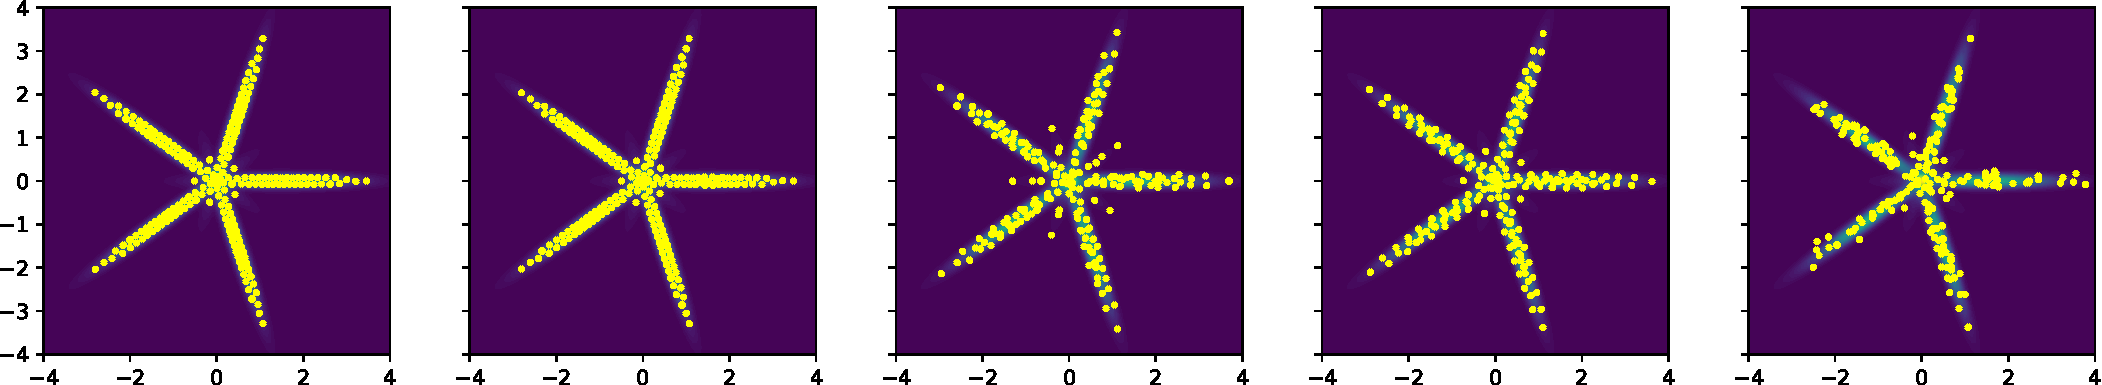
\includegraphics[width=\linewidth]{Star_compare}
\caption{ Particles obtained by various methods [200 particles]: (a) EVI-Im after 20 iterations, (b) Blob method (after 1000 iterations), (c) SVGD (after 1000 iterations), (d) matrix-valued SVGD (after 200 iterations) and (e) LMC (after 3000 iterations)}\label{fig:star}
%Particles obtained by various methods [200 particles]: EVI-Im after 20 iterations, Blob method and matrix-valued SVGD both after 1000 iterations; (b) cross-entropy v.s. number of iterations of the three methods.\label{fig:star}}
\end{figure}

SURE students will learn the foundations of variational methods and explore  and create new EVI algorithms by trying different combinations of divergence functionals and dissipation laws. 
They will develop new numerical schemes and build software based on them. 
SURE students will also explore new applications of the EVI algorithms in machine learning focusing on supervised learning models and generative learning models. 
They will work on interesting case studies with real-world data sets and problems. 


\subsubsection{Pattern Forming Problems in Physical and Biological Systems}
Once the machine learning algorithms aforementioned are fully developed, we will implement them in real physical or biological problems, in particular, pattern formation in non-equilibrium dynamical systems.  From
a mathematical point of view, studies of the pattern formation can be
formulated as moving boundary problems with interfaces separating
different physical  domains.  In the last few decades, theories,
experiments, and nonlinear simulations have contributed to gain a
better understanding of the mechanisms ruling the pattern selection,
in which interfacial instability is the central question. 

Interfacial instabilities occur when driving forces compete with resistive forces and typically result in the formation of complex patterns. Examples can be found in a wide
variety of systems, including filamentary microorganisms \cite{alain},
growing biofilms \cite{dockery01,Mattei2018}, tumor growth  \cite{MJ2020,Kara2018}, silica tubes forming in electrically-driven metal salt solutions \cite{steinbock03,steinbock16}, smoldering flame fronts
\cite{zik98,Kagan2008}, or lava flows \cite{balmforth00, griffiths00,Roman2021} in which
the interface itself is defined by a reaction or a solidification, and
driven by the expanding growth of the interior. Resistive forces include surface tension, viscous dissipation, bending, elasticity, and viscoelasticity.

There are a few critical parameters (e.g., flow field and initial interface configuration) that can  be estimated via machine-learning (ML) methods. These parameters may be spatial and temporal dependent and their values will be an output from ML algorithms. We formulate this estimation as a Constrained Multi-Output Learning problem as follows: suppose there are $T$ outputs, $y_1, \ldots, y_T$, and these outputs are related by a set of  $P$ equations, which link the available experimental data and simulation results: $\Gamma_p(y_1, \ldots, y_T)=0, p=1, \ldots, P$. For example, these equations will arise from matching the time evolution of interface sizes and shapes from simulation predictions with experimental measurements, which will be obtained by post-processing the images and videos of the  dynamical process. We aim to learn the $T$ outputs jointly (instead of separately) while satisfying the $P$ constraints. 

\begin{wrapfigure}{r}{0.66\textwidth}
%  \centering
  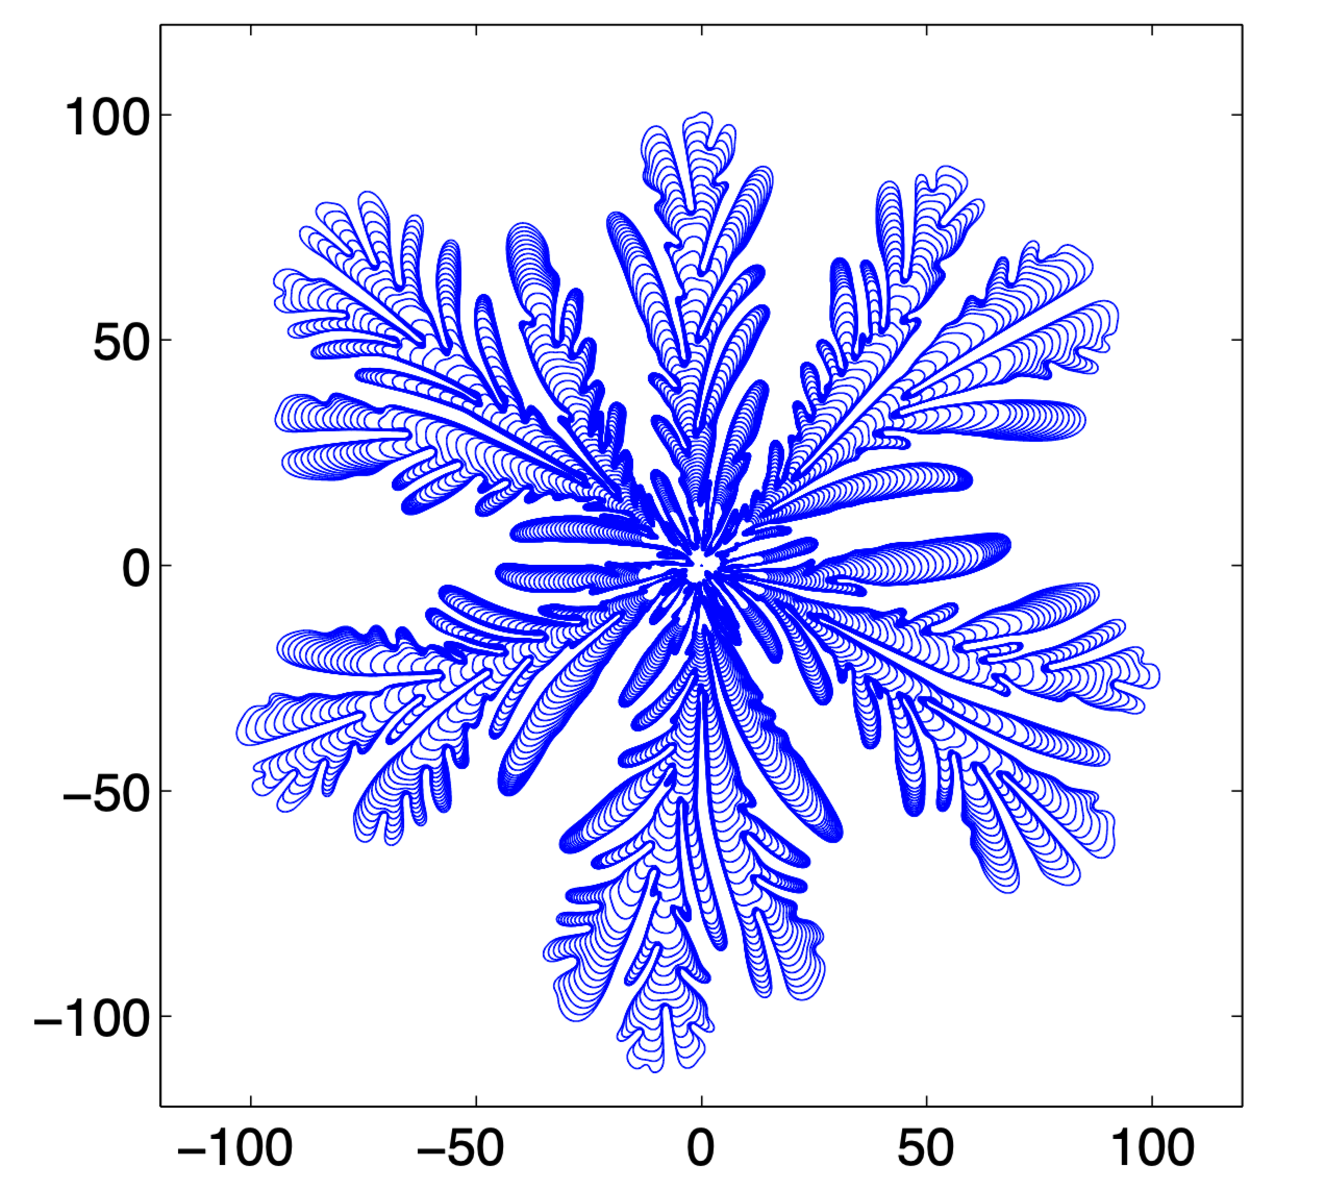
\includegraphics[scale=0.2]{Unstable}[a]
  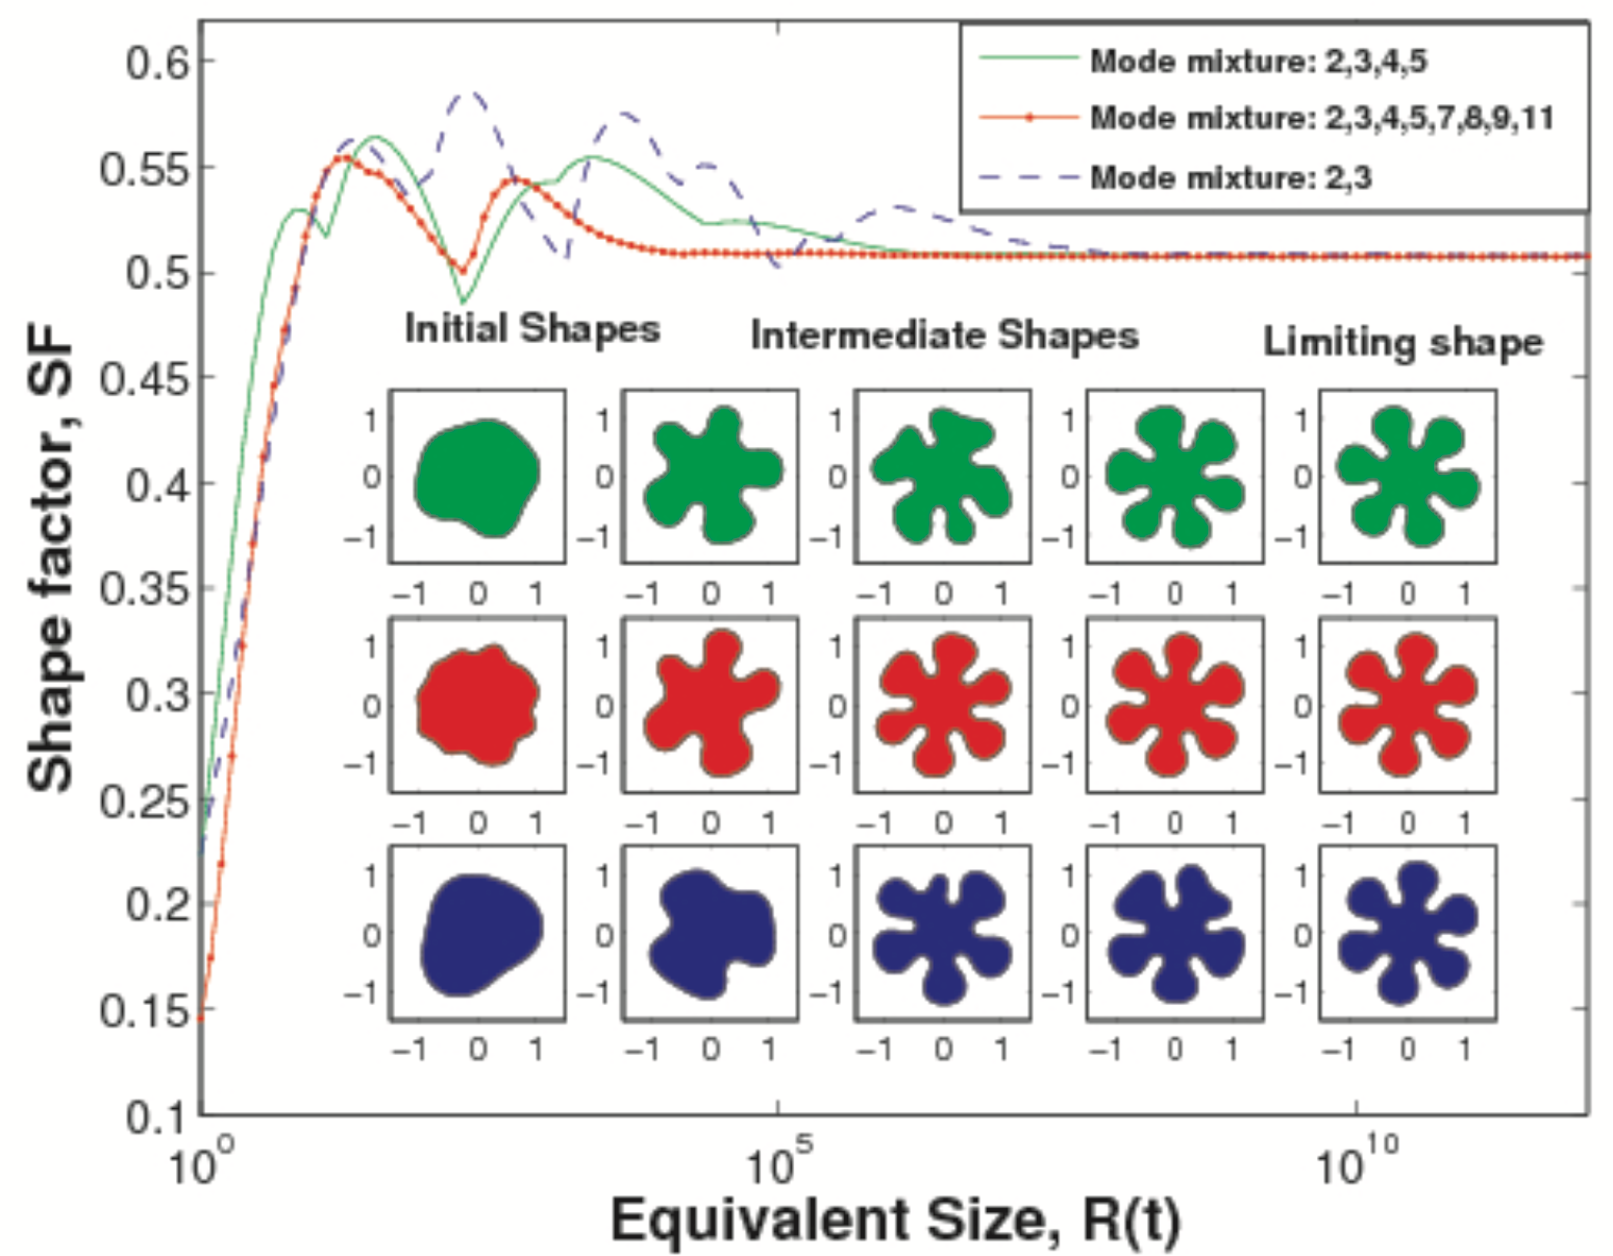
\includegraphics[scale=0.2]{Stable2}[b]
  \caption{An illustration of [a] unstable growth; [b] stable  dynamical equilibrium patterns with six-fold symmetry in a Hele-Shaw flow.}
  \label{figA}
  \end{wrapfigure}

 We propose a focused, coherent study of interfacial instabilities with an integrated analytical and numerical effort between faculty mentors' research groups. One sample project could be investigating a classic pattern forming system in fluid dynamics: viscous fingering in a Hele-Shaw cell \cite{saffman1986}. Our main goals are to investigate the nonlinear dynamics of interfaces and identify critical physical parameters (e.g., critical evolution time or size that an interface starts to equilibrate) via a ML approach such that a dynamical equilibrium state with certain symmetry can be achieved at a prescribed time or size. See Fig.~(\ref{figA})[a] for an illustration of unstable pattern development by repeated tip splitting process and Fig.~(\ref{figA})[b] for a six-fold self-similarly evolving pattern at dynamical equilibrium \cite{Li2009}. If time permits, we also plan to extend our research to avascular tumor growth using solvers recently developed in Li's group \cite{MJ2020}. The tumor problem involves more physical and biological parameters governing the dynamics and nutrient fields in tumor and  host tissues. We expect the developed machine learning algorithms to be more explorative of parameter space and to determine optimal parameter ranges for controlling the tumor-host interface.




%\begin{figure}[th!]
%  \centering
%  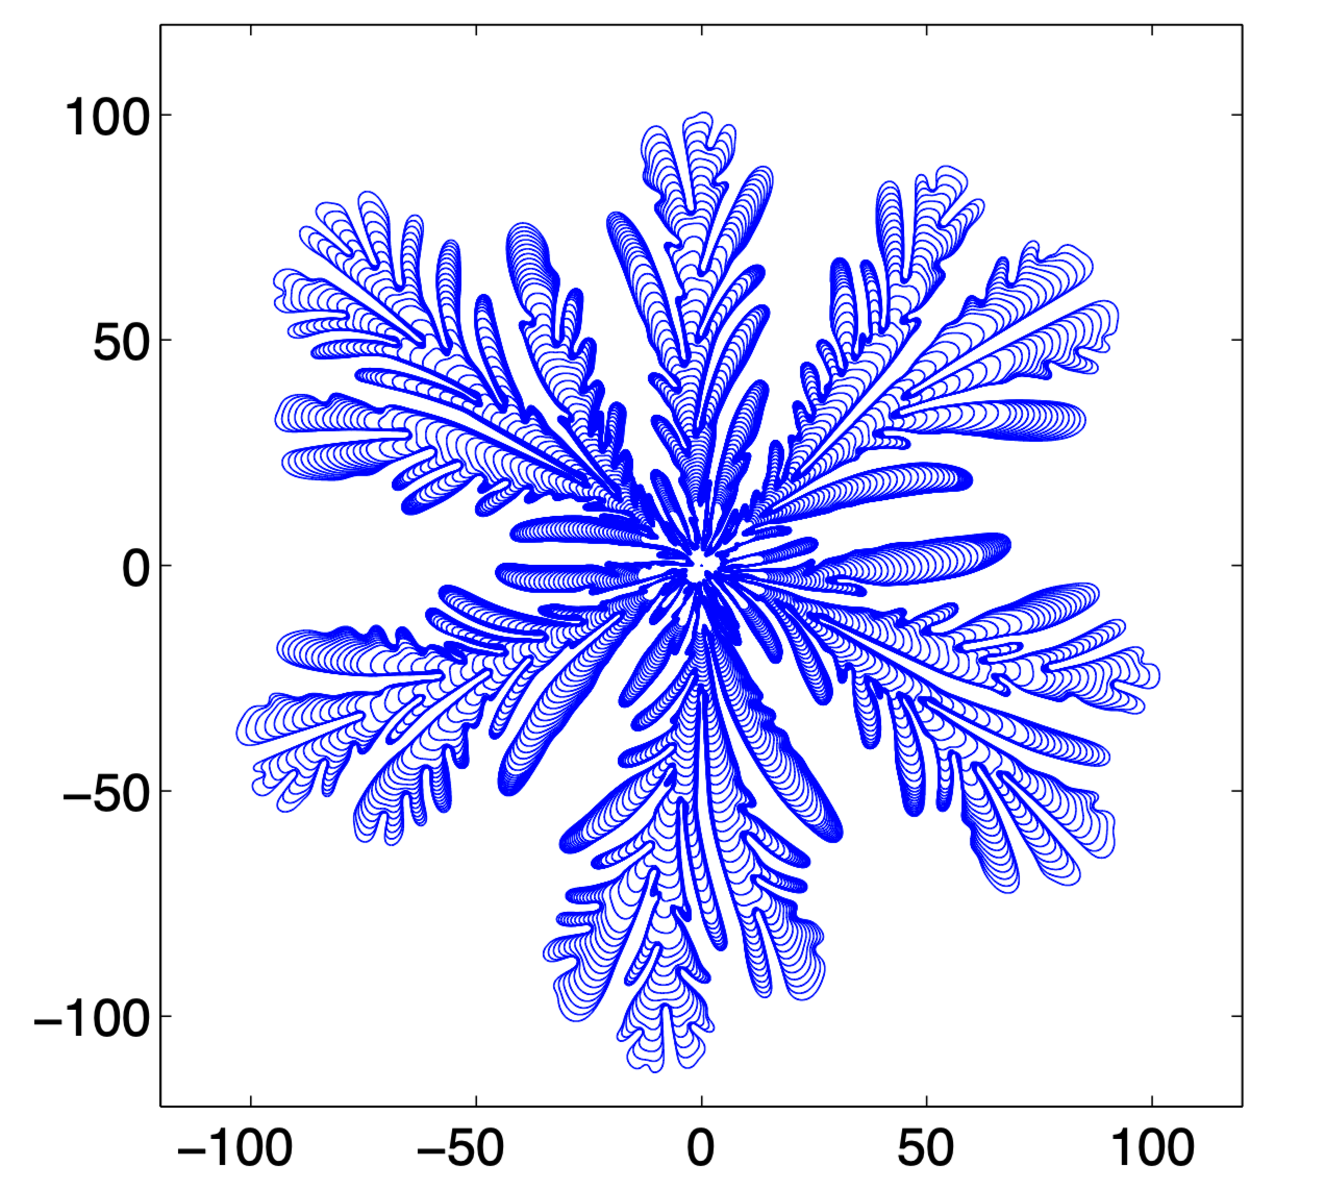
\includegraphics[scale=0.225]{Unstable}[a]
%  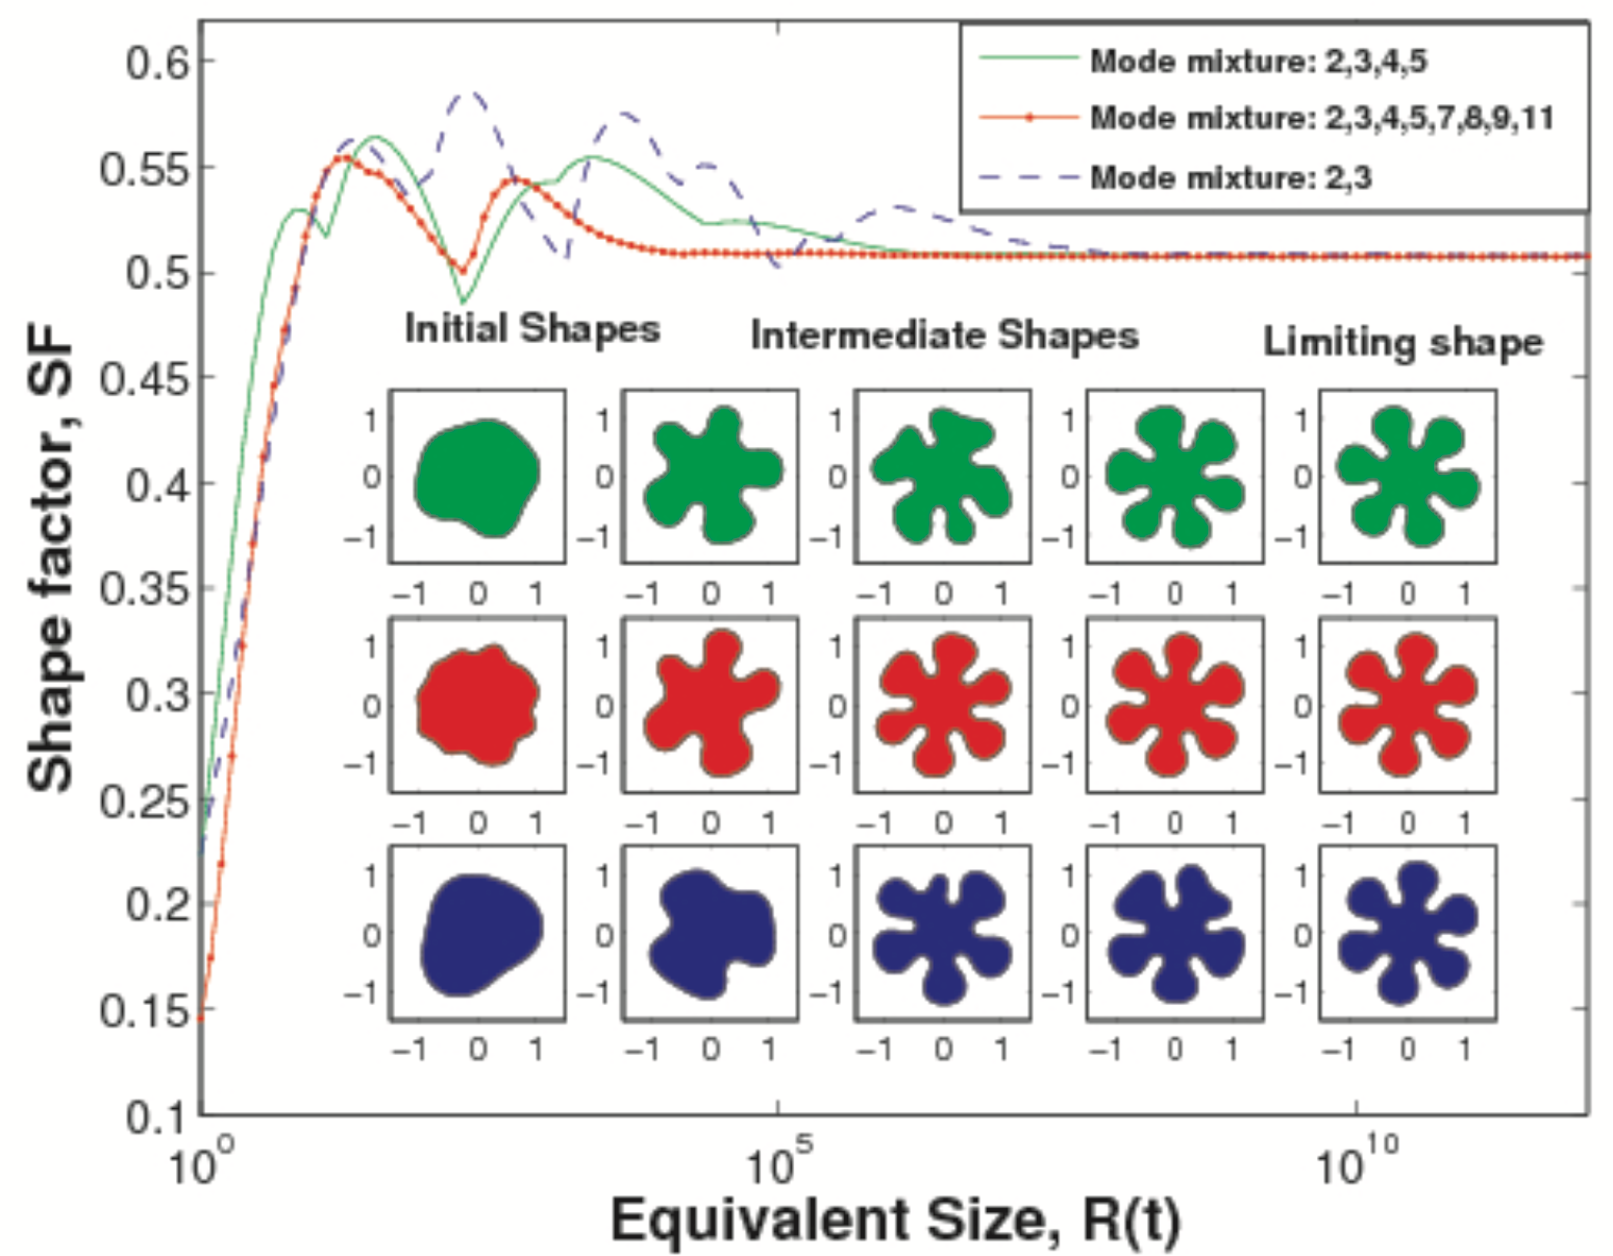
\includegraphics[scale=0.2]{Stable2}[b]
%  \caption{An illustration of unstable growth [a] and stable [b] dynamical patterns with six-fold symmetry in a Hele-Shaw flow.}
%  \label{figA}
%  \end{figure}


  


%There are many potential applications of this work due to the ubiquity of pattern-forming systems that are driven out of equilibrium. The interest in understanding the formation kinetics and the interplay of system parameters is to provide an understanding of growth and form in nature as well as to achieve improved control and efficiency in a variety of physical, biological and engineering systems. For example, in industrial oil recovery techniques, where process strategy is to inject fluids (water, supercritical $CO_2$, surfactants, etc.) into oil containing porous media to push out the oil, the main problem is that the interface between the injected fluid and the oil becomes unstable, and fingers of injected fluid grow and advance, instead of pushing the oil out. Thus, the time-dependence of the injection rate may play an important role in process efficiency, by ameliorating or enhancing instability. Many problems in biology also involve pattern-forming systems (e.g., bacteria colonies, biofilms, etc.) where the driving force (cell-proliferation, pressure, flow, etc.) and resistive forces (e.g., elastic membranes, production/destruction of extracellular matrix scaffolds) interact. We anticipate that the tools developed here may be adapted to provide insight into these problems.


The proposed sample project is expected to provide an understanding of growth and form for such problems, and our coupled mathematical and statistical machine learning approaches are also expected to have applications beyond the present context.  Students will receive interdisciplinary training while solving the proposed problems. % This research project can involve undergraduates from various disciplines and provides an opportunity for students to apply and develop their teamwork spirit, project management, communication, and ethical behavior skills. Specifically, 

The specific {\bf learning goals} for students are to be able to 
\begin{itemize}[leftmargin=.5cm]\vspace{-1ex}
    \item  Describe the proposed physical and biological problems and related principles governing the system; 
    \item  Explain the fundamental framework for developing mathematical models;
    \item  Implement their models in a computer; 
    \item  Explain their research findings.
\end{itemize}
The specific {\bf research goals} for students are to 
\begin{itemize}[leftmargin=.5cm]\vspace{-1ex}
    \item  Develop subroutines for their specific models and incorporate them in the developed codes;
    \item  Explore parameter spaces using basic statistic or ML tools and design  targeted simulations;
    \item  Perform data analysis and post-process after simulations in terms of deliverable plots and videos.
\end{itemize}

%\begin{itemize}
%    \item students will learn the fundamental framework for developing mathematical models;
%    \item students will learn the implementation of mathematical models in a computer;
%    \item students will learn the analysis (and post-process) of data in terms of plots and videos.
%    \item students will be able to explore parameter spaces using basic statistic or machine learning tools.
%\end{itemize}



\subsubsection{ REU in Computational Finance with Heterogeneous Big Data}

The purpose of this proposed REU in computational finance with heterogeneous big data is to prepare our undergraduate students in Applied Mathematics or Computer Science to become innovative and ambitious members of our society. Successful outcomes would include students applying their knowledge acquired from coursework or independent research reading,  designing data-driven solution approaches, to alleviate important global problems such as financial crisis associated with climate change, harmful large-scale industrial practices, widespread public health, or environmental issues such as an epidemic.  The key components of this SURE program would include real-world (multiple) un/semi-/structured time-series data from finance and other areas; introduction to the literature on existing cutting-edge scientific theories and modern computational tools; as well as an emphasis on rigorous evaluation of analytical results with different metrics. 

One example would be the impact of ESG (environment, sustainability, and government) risk factors on the financial health of companies. There is no doubt that extreme weather events such as floods could wipe out many buildings and infrastructure in the affected areas, leading to a huge financial loss of many companies that have businesses there, possibly resulting in immediate failures to fulfill their financial obligations to business partners and global financial participants who own financial assets issued by these companies. Nevertheless, existing definitions of ESG measures the input data collection process, and scoring methodologies, to name a few, are often very unclear to various stakeholders, if not controversially biased (see, for example, \cite{reiser2019buyer}). In some cases, their connections to company default data are hard to come by. A meaningful REU project would engage students to critically examine some existing ESG scores (e.g., \cite{friede2015esg}); hypothesize their relationships with more readily available, observable market information such as company share prices or bankruptcy data \cite{pedersen2020responsible, fatemi2018esg}; formulate the problems in mathematics as (stochastic) dynamical systems or optimization; perform statistical analysis, discretization, or extend more powerful explanatory/prediction models of company default such as \cite{jarrow2005default}; and analyze the resultant errors or accuracies. 

In such a project, students would be exposed to important open problems in the emerging area of sustainable finance and become motivated to apply mathematical principles and statistical techniques from courses they had taken. They would come to identify knowledge gaps of their own or the interdisciplinary disciplines and become motivated to improve or even invent new scientific tools and algorithms for solving these challenging problems.


\subsubsection{Smarter Monte Carlo Sampling}
Multivariable integrals arise in Bayesian inference, quantitative finance, and uncertainty quantification.  When the number of variables, $d$ is more than a few, tensor product rules are impractical because the rate of convergence, $\Order(n^{-r/d})$, where $n$ is the number of sampling points, degrades catastrophically with $d$, even if $r$, the smoothness of the integrand and the associate method is substantial.  The most computationally efficient methods are Monte Carlo methods, where the integral of interest is interpreted as the expectation (or population mean) of a function of a (uniform) random variable, which is then approximated by a sample mean.
$
    \int_{\Omega} g(\bt) \, \dif \bt = \int_{[0,1]^d} f(\bx) \, \dif \bx = \Ex[f(\bX)] \approx \frac 1n \sum_{i=1}^n f(\bx_i).
$

The root mean square error using $\bx_1, \bx_2, \ldots \IIDSim \calu[0,1]^d$ is $\std(f(\bX)) n^{-1/2}$, which translates into a computational cost of $\Order(d\var(f(\bx))\varepsilon^{-2})$ to obtain an approximation with absolute error no greater than $\varepsilon$. The term $d$ accounts for the cost of evaluating $f$, which is assumed to be proportional to the number of variables, $d$.

There are several ways to decrease the cost of computing an acceptable approximation to the integral.  Quasi-Monte Carlo (QMC) methods \cite{DicEtal14a} replace IID sample points by low discrepancy (LD) sample points, such as Sobol' or lattice points, reduces the cost to $\Order(d\norm{f}\varepsilon^{-1+\delta})$ for arbitrarily small, positive $\delta$, where now the size of integrand is measured by a norm that requires a bit more smoothness than IID Monte Carlo. 

Multi-level methods write the integral for large or even infinite $d$ as a telescoping sum involving integrals of increasing dimension. 
For many problems of interest, such as those where $f$ represents the payoff of an exotic option, one can use a large number of samples for the terms with small dimension and a small number of samples for the terms with large dimension so that the total computational cost now loses its $d$ dependence and becomes $\Order(\norm{f}\varepsilon^{-1+\delta})$.
 
\begin{wrapfigure}{r}{0.56\textwidth}
	\centering
	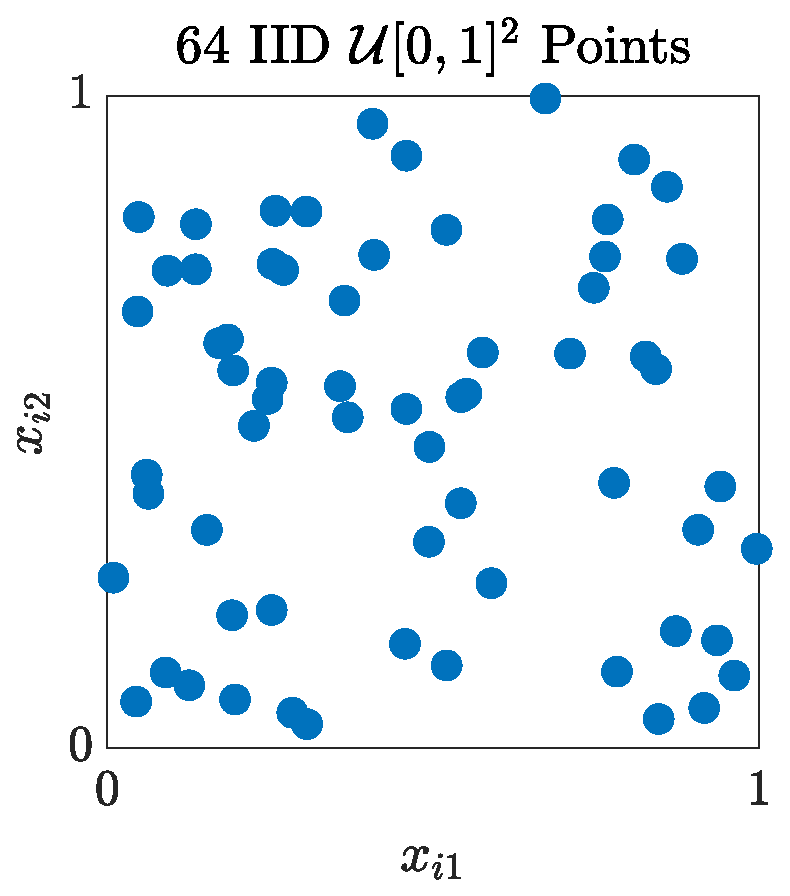
\includegraphics[height = 4.5cm]{IIDPoints.eps} \quad
	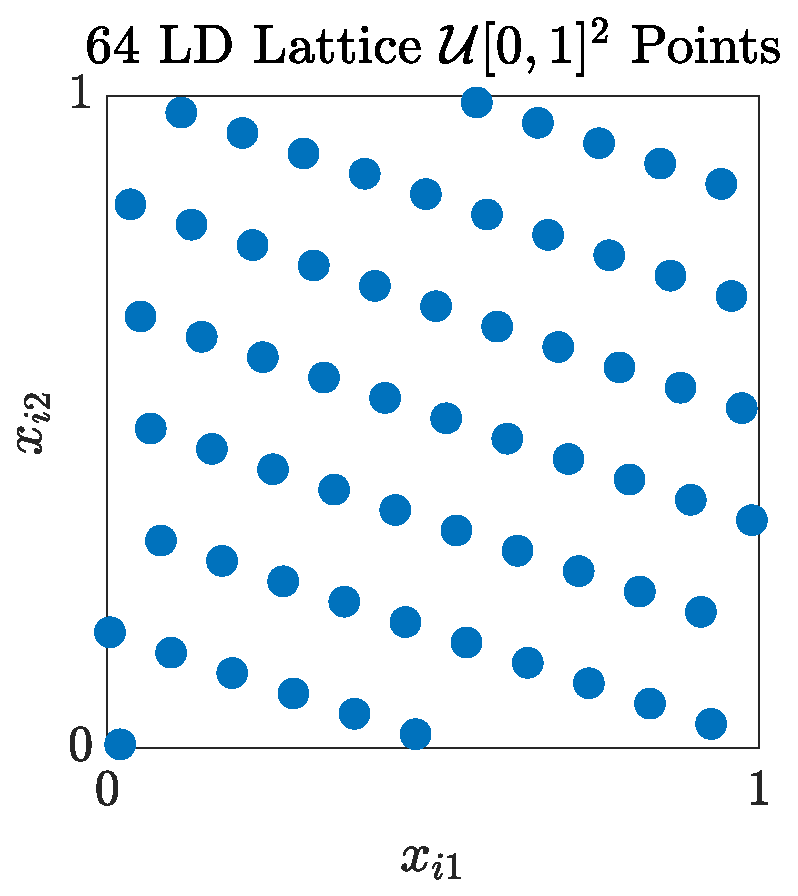
\includegraphics[height = 4.5cm]{ShiftedLatticePoints.eps}
	\caption{IID points and LD lattice points.  The LD points have fewer gaps and clusters of points than the IID points. \label{fig:iid_vs_ld}}
\end{wrapfigure}


Finally, the variable transformation from the original integral of $g$ to the final integral $f$ is non-unique.  Clever transformations, which may be regarded as importance sampling, make $\norm{f}$ smaller.  The integrands, $g$, in Bayesian inference problems are typically quite peaky, and importance sampling may drastically reduce the computational cost.

SURE students will explore one or more of these methods for more efficient Monte Carlo sampling in the context of QMCPy \cite{QMCPy2020a,QMCBlog}, an open-source quasi-Monte Carlo library developed by Hickernell, Choi, Ding, PhD student Sorokin and collaborators. The goal of the SURE projects will be to expand the menu of use cases for quasi-Monte Carlo, e.g., for efficient evaluation of acquisition functions in Bayesian Optimization and extending the work of Zhang \cite{Zha21a} in using QMC methods for Bayesian inference. 



\subsubsection{Pricing Options by Quasi-Monte Carlo (QMC) with Median Estimator}

Students in this project should have a basic understanding of statistics, such as mean, median, and variance. Calculus I and II are also required. Experience in programming will be preferred.

The sample mean is a good estimator of the population mean. However, the mean is easily affected by the outliers. Pan and Owen proposed a median-of-means approach using randomized digital nets to estimate an integral with a smooth integrand in \cite{SPAMOM22} and obtained an outstanding convergence rate. Inspired by this work, Goda and L'ecuyer studied a new construction-free median QMC rule with lattice points in 
\cite{CFMQMC} and obtained some excellent results. In this project, the students will implement similar ideas to solve the option pricing problem by QMC.

In this project, students will learn how to price options by regular QMC methods and combine them with the median-of-means approach. They will start from the European or Asian options, exercised only at the expiry of the contract. They will make a lot of simulations and comparisons between the traditional and new ways.

SURE students will better understand the differences between mean and median and know how to choose the estimator appropriately. More than that, they will learn and implement the QMC method in other research areas they are interested. The project will also enhance their programming skills through the simulation process. 













\section{The Research Environment}


 
\subsection{The Host Institute}

Illinois Institute of Technology is a private research university with around 19\% minority and 37\% female students. Illinois Tech is a diverse and welcoming community, featuring a campus with students from 89 countries and all 50 states. In 1890 the university was founded to lift people of all backgrounds with an education that would help them meet the needs of their age. Since its founding, Illinois Tech has inspired student researchers to see beyond the visible, push the boundaries of what is possible, and stretch the powers of the imagination. The College of Computing
and the Department of Applied Mathematics at Illinois Tech offer programs to involve students
in research, especially in undergraduate research. The department always provides independent study to undergraduate students. In 2019, the summer elevated research courses started. In addition, beginning in January 2021, SoReMo Initiative (Socially Responsible Modeling, Computation, and Design) offers semester-long research fellowships that provide unique interdisciplinary research opportunities for students who want to apply computational modeling and design skills to solve a social issue. The department of Applied Mathematics organized a pilot program of summer undergraduate research since 2021. The details can be found in Section \ref{sec:SURE}.


\subsubsection{Organizations' Commitments to the REU site}
The Department of Applied Mathematics and the College of Computing at Illinois Tech will strongly support the program. The department has committed to providing SURE participants with office space, discussion, tutorial and presentation classrooms, and access to computer equipment, printers, and the internet at no charge. Three graduate students will help with the tutorial/lab sessions each year.
The Office of Enrollment will fully support the application process, admission, registration, and on-campus housing. 
The Office of Research Integrity and Compliance will provide a presentation on \emph{Responsible Conduct of Research} to all SURE program participants. The Office of Title IX Compliance will help all SURE students, faculty mentors, and graduate students understand how to prevent sexual harassment and respond if it occurs.

SURE students
will reside in Illinois Tech McCormick Student Village or State Street Village. The furnished halls are suite-style, allowing students to interact with one another outside of the program. The halls provide WiFi, laundry
lounges, and meeting rooms. The McCormick Tribune Campus Center provides a large variety of dining options. Illinois Tech will give access to all facilities to the SURE participants. 




\subsection{Faculty Mentors}
\hypertarget{YDlink}
PI Yuhan Ding (\YD) will serve as Program Director to oversee the management of the SURE
program. \hypertarget{FHlink} Co-PI Fred Hickernell (\FH) will serve as Co-Director to assist
with day-to-day activities and monitor the research progress of the students during and after the program. There are three senior personnel, \hypertarget{SCTClink}Sou-Cheng Choi (\SCTC), \hypertarget{LKlink}Lulu Kang (\LK), and \hypertarget{SLlink}Shuwang Li (\SL), from the Department of Applied Mathematics in the College of Computing at
Illinois Tech. Three are women faculty (\YD, \SCTC, and \LK). Each year, three out of five will serve as faculty mentors.
 All faculty mentors are
active in their fields and have extensive experience mentoring undergraduate students, ensuring the quality of mentoring activities and the program's success. 


\YDNote{The introduction focuses more on the undergraduate mentoring}

\noindent \underline{\textit{PI Yuhan Ding}} first mentored an undergraduate capstone project in 2018 as a co-adviser. In addition, she provided tutorials for MATLAB and LaTeX to undergraduate students many times. In 2019, she advised three students in a summer research course. All of them are in master’s programs now. Starting in 2021 fall, she served as a core member of the SoReMo Initiative of Illinois Tech, which provides unique interdisciplinary research opportunities for students who want to apply computational, modeling, and design skills to solve a social issue. She supervised one undergraduate SoReMo fellow and reviewed his final report. She also provided feedback on other fellows’ projects during the biweekly presentation. In the summers of 2021 and 2022, she coordinated the pilot program.

\noindent \underline{\textit{Co-PI Fred Hickernell}} has supervised 16 PhD students, a handful of master's thesis students, and a couple of dozen undergraduate research students.  He has authored over a hundred refereed publications, including \cite{ChoEtal22a,HicEtal14b,LiHic03a,SonRidFasHic10a} with five undergraduate students.  Undergraduate students mentored by \FH have gone on to graduate programs at Johns Hopkins, Princeton U, RPI (an African-American), U Illinois Chicago (a Latina), and UCLA. \FH is a Fellow of the IMS and has served on the editorial boards of several computational mathematics journals. 

\noindent\underline{\textit{Sou-Cheng Choi}} has served as a mentor or research co-advisor to more than 8 doctoral, 4 master’s, 13 undergraduate from Illinois Tech, the University of Chicago, University of Illinois at Urbana-Champaign, through Illinois Tech's   research seminar courses, Summer research programs, internships related to design of mathematical algorithms, machine learning and big data with applications in investment science, corporate finance, or  social sciences at Illinois Tech and University of Chicago since 2013. 
She also guided a high school student from IMSA in 2016 and now he is a double major in mathematics and computer science at Harvey Mudd College.



\noindent \underline{\textit{Lulu Kang}} has mentored six applied math and computer science undergraduate students on various topics in statistics and machine learning since 2018. Most of them were female and/or minority students. In the past decade, she has advised eight M.S. students and two PhD students on their theses on various topics in statistics and related areas. \LK has also been active in community outreach by advising three high school students on applied statistics and machine learning projects. 
\LK has worked on various areas in Statistics and Machine Learning, including uncertainty quantification, statistical design and analysis of experiments, Bayesian inference, etc. 
\LK has developed and taught many statistical courses including Statistical Learning, Bayesian Computational Statistics, and Regression and Forecasting, etc. She is also the co-founder and Associate Program Director of the Data Science Program at Illinois Tech. \LK is currently the associate editor for journals \emph{\SIAM/American Statistical Association (ASA) Journal on Uncertainty Quantification} and \emph{Technometrics}.

\noindent \underline{\textit{Shuwang Li}} has supervised eight PhD students and five master's students with thesis option. \SL also mentored six undergraduates including students from other universities (doing research with \SL during summer). The two female undergraduate students went to graduate schools at Columbia and Ohio State,  and one of them published a joint paper with \SL at {\it \SIAM Undergraduate Research Online} (SIURO). 
\SL is an expert in the theoretical analyses and
long-time adaptive simulations of free boundary problems in  fluids and
materials. \SL developed a novel time-space
rescaling scheme that enables one to simulate evolving interfaces for much
longer times than had been previously possible, which led to the discovery of new nonlinear
phenomena: self-similar universal patterns in growing crystals and Hele-Shaw  flows. \SL also incorporates advanced numerical techniques on interface problems into special topics that are accessible to undergraduates. 

 


\section{SURE 2021 and 2022}
\label{sec:SURE}
A summer undergraduate research experience program (SURE) with an internal fund started in the 2021 summer. 
\begin{figure}[h]
    \centering
    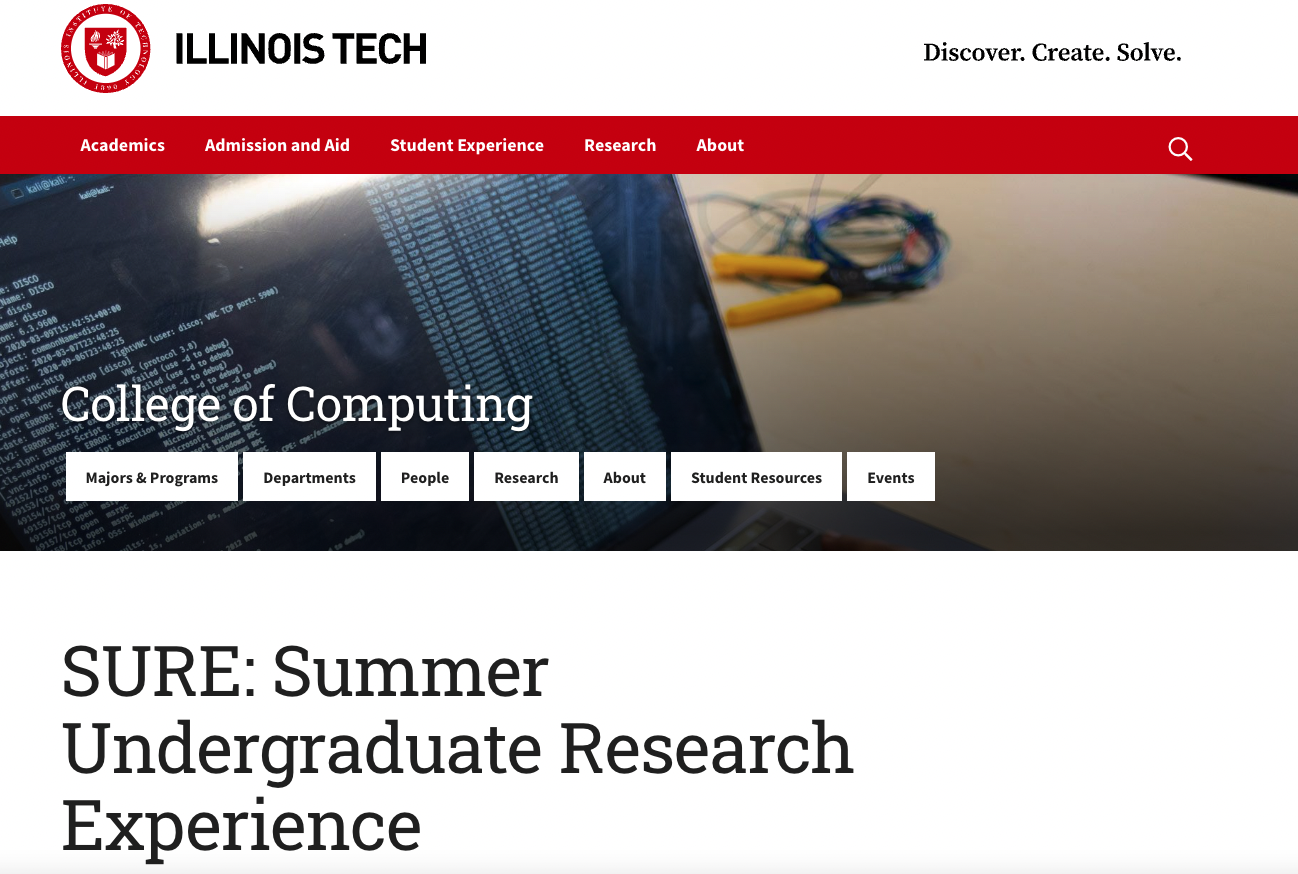
\includegraphics[width=0.35\linewidth]{SUREWebsite.png}
    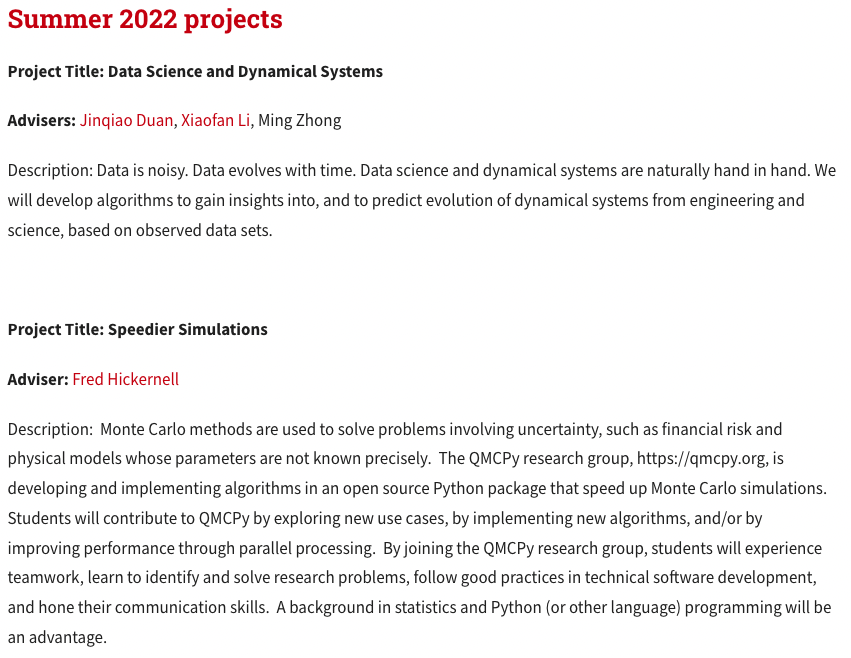
\includegraphics[width=0.3\linewidth]{SUREProgram.png}
    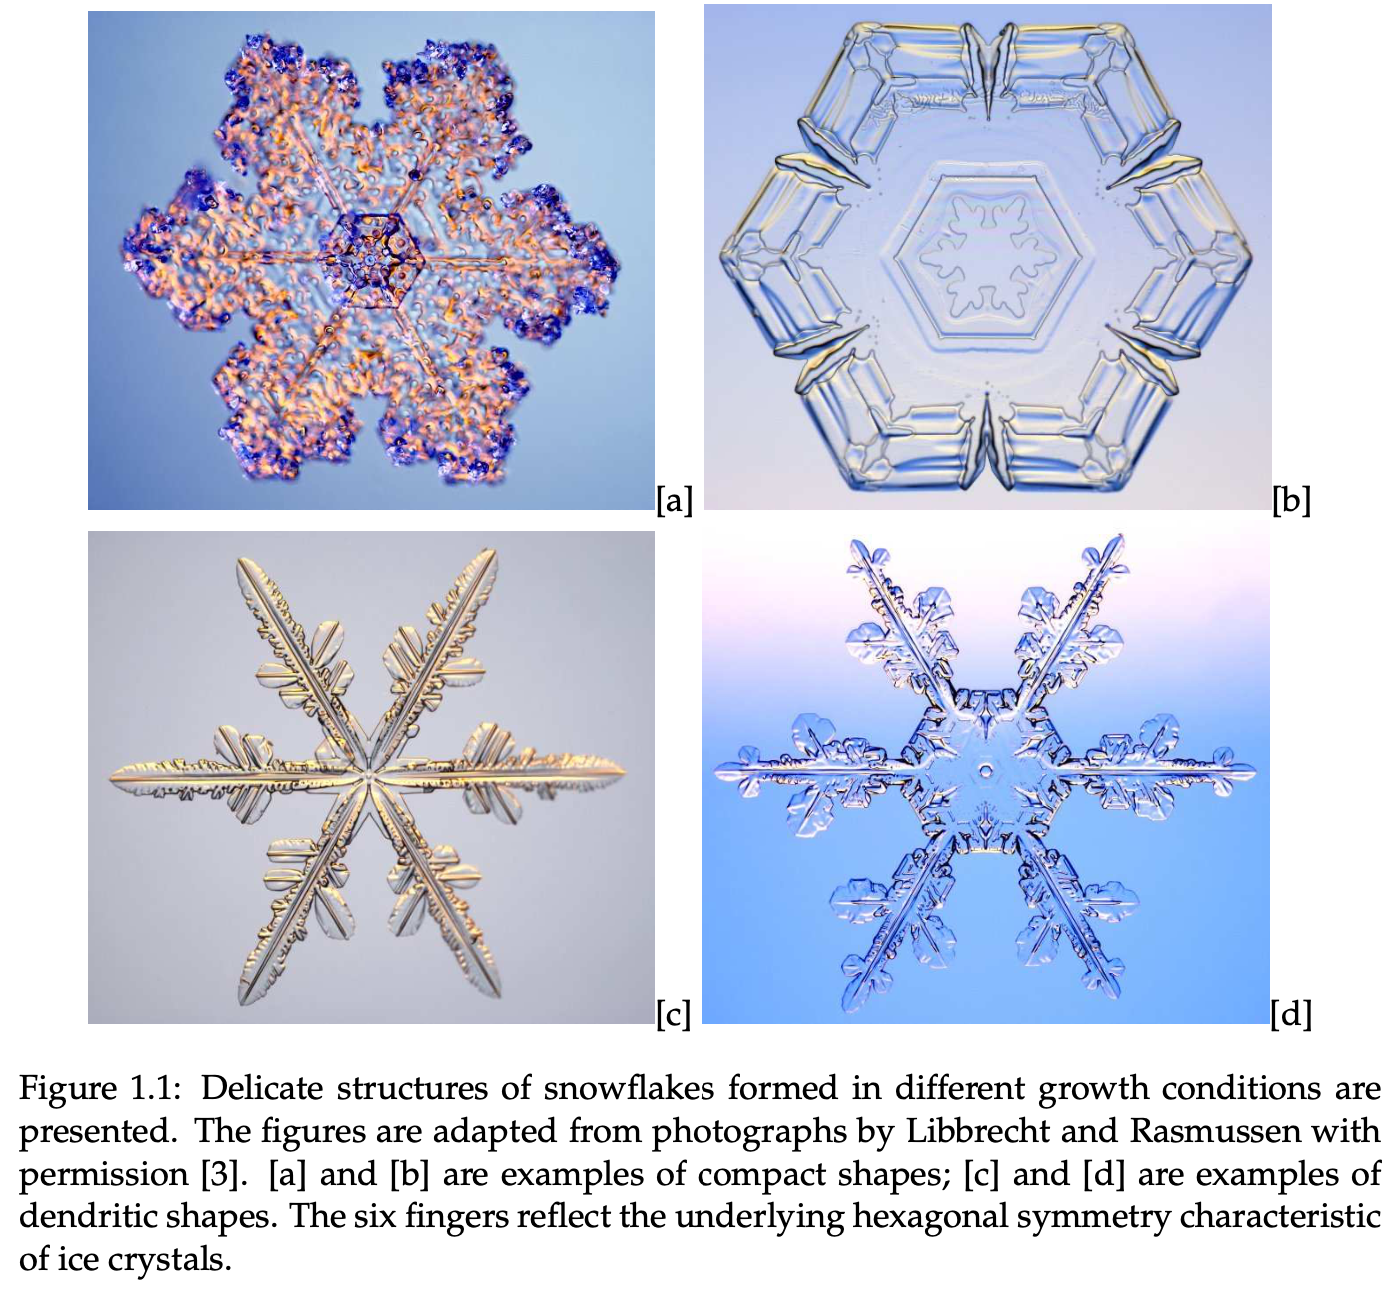
\includegraphics[width=0.25\linewidth]{IceCrystal.png}
    \label{fig:SUREWebsite}
\end{figure}


A \emph{seven-week} SURE program was hosted remotely in 2021, which involved \emph{six faculty mentors and seven undergraduate students}. This program was a collaboration between the departments of applied mathematics and computer science. \YD, the program coordinator, handled the selection of students and mentors, coordination of hybrid gatherings, social activities, and final presentations. \FH, \LK, and \SL served as mentors. \emph{Two undergraduates were racial minorities, four were female, one was a sexual minority, and three were first-generation college students.} Two SURE participants are in graduate programs. One of them is a Ph.D. student of Illinois Tech. The student who worked with \LK is still working with her during the semester.

In 2022, an \emph{eight-week} program which involved \emph{four faculty mentors and four undergraduate students} was hosted hybrid. \YD still served as the program coordinator. \FH, \LK, and \SL served as mentors. \emph{One of the undergraduates was a racial minority.} All students will keep working on their projects in the coming semester. Two SURE students attended the research poster day at Illinois Tech in August. 
All SURE students provided very positive feedback about the program. The detailed program information and comments from the participants can be found in \cite{SUREWeb}.

\begin{figure}[h]
    \centering
    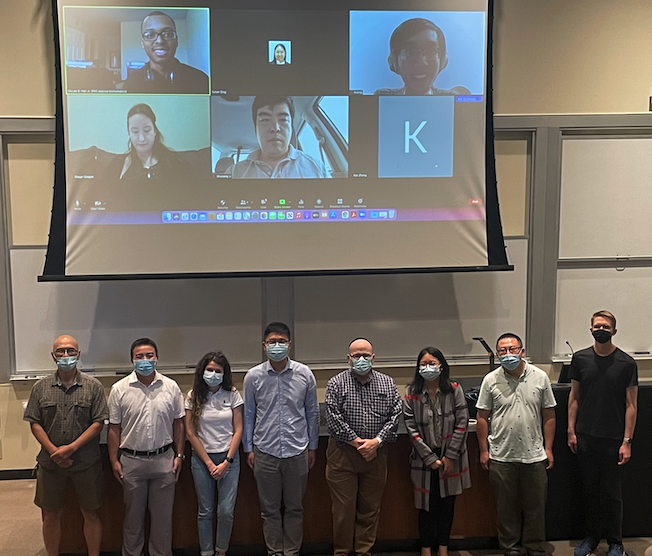
\includegraphics[width=0.3\linewidth]{SURE2021.pdf}
    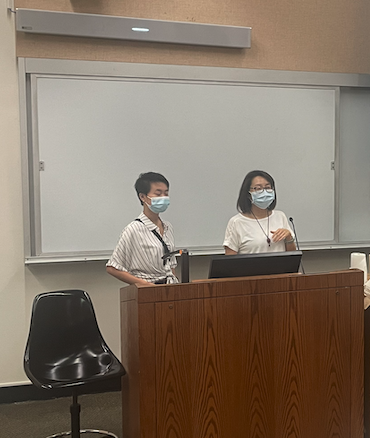
\includegraphics[width=0.3\linewidth]{SURE2021Midterm.pdf}
    \includegraphics[width=0.3\linewidth]{SURE2021Final.pdf}\\
    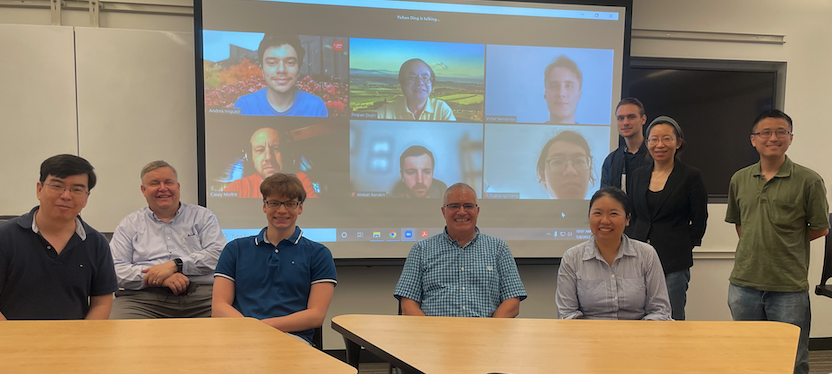
\includegraphics[width=0.3\linewidth]{SURE2022Final.pdf}
    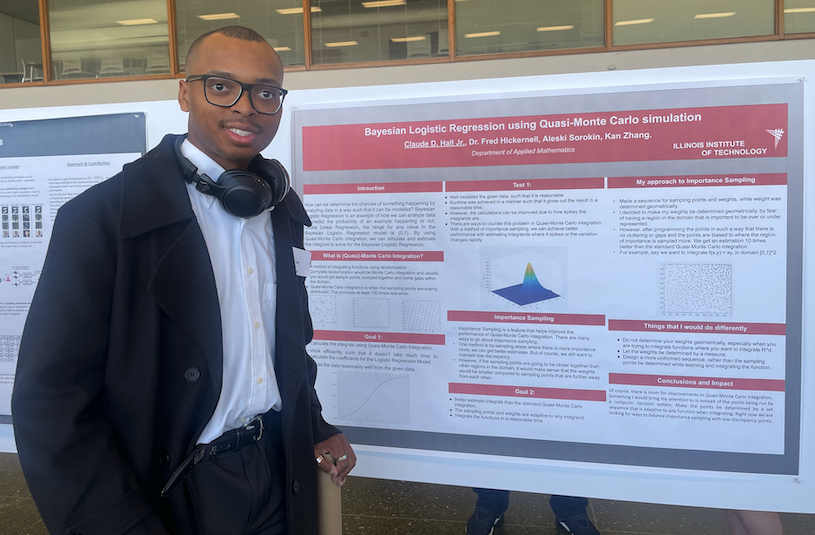
\includegraphics[width=0.3\linewidth]{Poster1.pdf}
    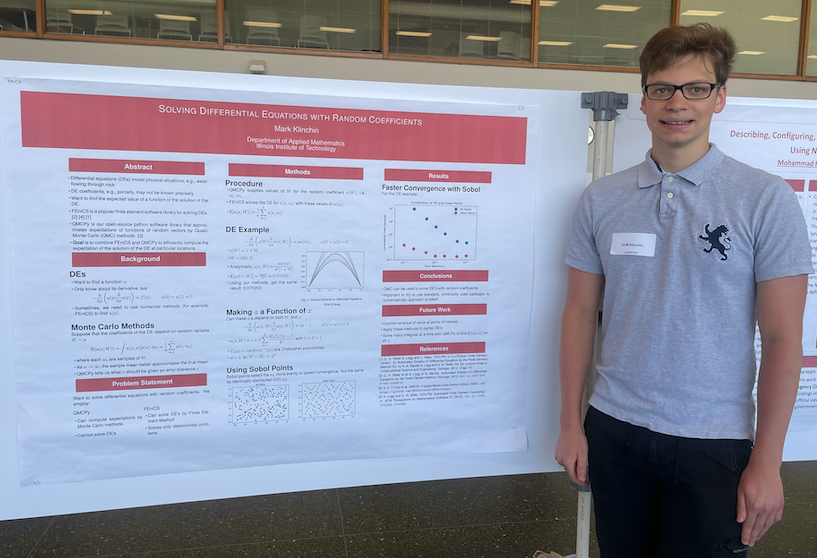
\includegraphics[width=0.3\linewidth]{Poster2.pdf}
    \caption{SURE Events}
    \label{fig:SUREevents}
\end{figure}



\section{Student Recruitment and Selection}

\subsection{Student Recruitment} 


\YDNote{Describe the experience we did in SURE and the improvement part}
 In the first year, the official recruitment will start after getting a notification from NSF.
 In the following years, the recruitment will start in September. The SURE website
 \cite{SUREWeb} will release important information about the program, including the program's start date and application deadline, program requirements,  all available projects, faculty mentors, a link to the application system, etc. In the meantime, the URL of the program’s
website \cite{SUREWeb} will be posted in the list of NSF-funded REU Sites and the websites of all Illinois Tech undergraduate research programs.

PIs will distribute a well-designed flyer to our collaborators MSU, CSU, NEIU,  and Wheaton College.
The PIs will also attach the brochure to emails sent to
chairs and undergraduate mentors in Applied Mathematics and Statistics at institutions in the US, especially
\MSIs and research-limited institutions, with a request to distribute the flyer to their undergraduates. 
In addition, the flyer
will be posted on publications associated with ACM/IEEE chapters, Focus of \hypertarget{MAAlink}{Mathematical Association of America} (\MAA), \hypertarget{AWMlink}{Association of Women in Mathematics} (\AWM)
Newsletter, \hypertarget{NAMlink}{ National Association of Mathematicians} (\NAM) Newsletter, and Math Horizons and also in the Illinois Tech campus newspaper, bulletin, and electronic boards.

More than that, the faculty mentors will visit our collaborators, give seminars or colloquium talks, and promote the program. 
Faculty mentors will attend some regional and national conferences, such as
the annual  \hypertarget{JMMlink}{Joint Mathematics Meetings} (\JMM), \MAA MathFest, \NAM, and other conferences for minority students, for example, meetings of the Society for the Advancement of Chicanos/Hispanic and Native Americans in Science  (SACNAS) and 
\AWM  to advertise the program and distribute the flyer. 

\YDNote{Add more out-reaching events; maybe cross the state}

\subsection{Application and Selection} 
Applications received before the 2nd Monday of February will be given full consideration, but applications will be accepted until all slots are filled. Decisions and offers will be made by the end of February. Students will be asked to respond to the request within two weeks of notification but no earlier than the March 8 common deadline for mathematics REUs. If any student declines, another applicant will be offered an alternate offer. 
Each applicant will start an application from the link on the program’s
website and submit the following materials: 
Contact information, citizenship status, expected graduation date, GPA, college transcripts (especially courses and computer skills related to the program),
optional minority status, optional sexual information, and optional first-generation-in-college status;
At least one recommendation
letters from faculty members; 
One essay regarding their experience with, and interest in, research and in particular research projects, reasons for being involved in this program, their future
education, career plans, and how they feel the program will facilitate their goals. 

A recruitment committee of faculty mentors will review applications and rate the students. Students
will be rated based on GPA, courses, skills related to the program, letters of recommendation,
research interests, career objectives, and demographic information. Faculty mentors
will develop a rubric to guide the selection
process. This rubric will focus the team on relevant student prior performances, aiming to reduce the
influence of unconscious bias. Based on the
discussions with highly qualified students and priorities given to those from the underrepresented
groups and research-limited institutions, ten students will be selected.


\section{Student and Mentor Professional Development}
\subsection{Student Professional Development}
\FH, as the Vice Provost for Research, will invite a colleague in the  Office of Research to make a presentation on \emph{Responsible Conduct of Research (RCR)} to address: (1) the integrity of research; (2) authorship;  (3) good behavior
and quality research conduct; (4) bad behavior such as fabrication of data, falsification of data and
plagiarism; and (5) the ethics associated with the responsibilities of mentoring, peer relationships, review \& publication, data management, and conflicts of interest. After the presentation, we will have group discussions with some scenarios to help students understand RCR better.
All students must complete one RCR training course provided by Illinois Tech through CITI.  In addition, we will invite a librarian at Illinois Tech to give a presentation regarding the \emph{reproducible research and open scholarship} to address: (1) the advantages of  reproducible research, (2) how to make your research work publicly available to others, and
(3) how to share your raw data or code.

A workshop series on application and admission for graduate programs and strategies for success in academic careers will be organized from Week 6 to Week 8. The series provides SURE students with more information regarding graduate study and prepares a solid background to pursue an advanced degree.  During the following academic year, SURE participants will be connected to faculty mentors and graduate students through regularly scheduled Skype/Zoom meetings and emails as they continue to finalize their manuscripts for publication. Faculty mentors will submit papers to conference proceedings and academic journals for publication. In addition, SURE will financially support the participants to present their work at professional conferences and workshops, especially venues that host undergraduate research sessions, such as \MAA MathFest, \JMM, and \hypertarget{SIAMlink}{Society for Industrial and Applied Mathematics} (\SIAM) annual meeting. Faculty mentors will advise students to take classes that reinforce or supplement the topics covered during the summer program, take courses such as an independent study or senior thesis to obtain research credit for their project, and apply for graduate study.
The participants also have a chance to do long-term research with the guidance of their mentors.

 \subsection{Mentor Professional Development}
The colleague in the Office of Research Integrity and Compliance will also make a presentation on efficient mentoring for all faculty and graduate student mentors to address: (1) case studies
of mentor abuses; (2) responsibilities of mentors; (3) the strength and weakness of different types of students and how these can challenge mentors, etc. In addition, \YD will conduct at least one face-to-face RCR discussion session. \YD will hold a formal RCR instruction session or conduct informal RCR instruction as topics arise during the natural course of research activities with other faculty mentors and graduate students. 





\subsection{Creating a Safe and Respectful Environment} 
We will invite Virginia D.\ Foster, Title IX Compliance Coordinator, to present Title IX Compliance to all the SURE students, faculty mentors, and graduate students about
(1) matters related to sexual harassment,
(2) the university policy regarding matters related to sexual harassment,
(3) the appropriate way to react
(4) expectations of behavior on campus. Afterward, Virginia will provide several scenarios and lead a group discussion to help students understand Title IX better. 


\section{Project Evaluation and Reporting}
The proposed external evaluation will be led by \hypertarget{GPlink}{Dr.~Gorjana Popovic} (\GP) (see supplementary document for GP’s expertise). She will work directly with the SURE team to implement the evaluation plan.  \GP will author the annual evaluation report including results and improvement recommendations. The SURE team will respond to these reports in written form, documenting
the impact on the program. The conceptual model of the evaluation is shown in Figure \ref{fig:my_label}. \GP will also audit the implementation process
to ensure the program is implemented with integrity. Both quantitative and qualitative analyses are planned as follows.

\begin{figure}[tbh]
    \centering
    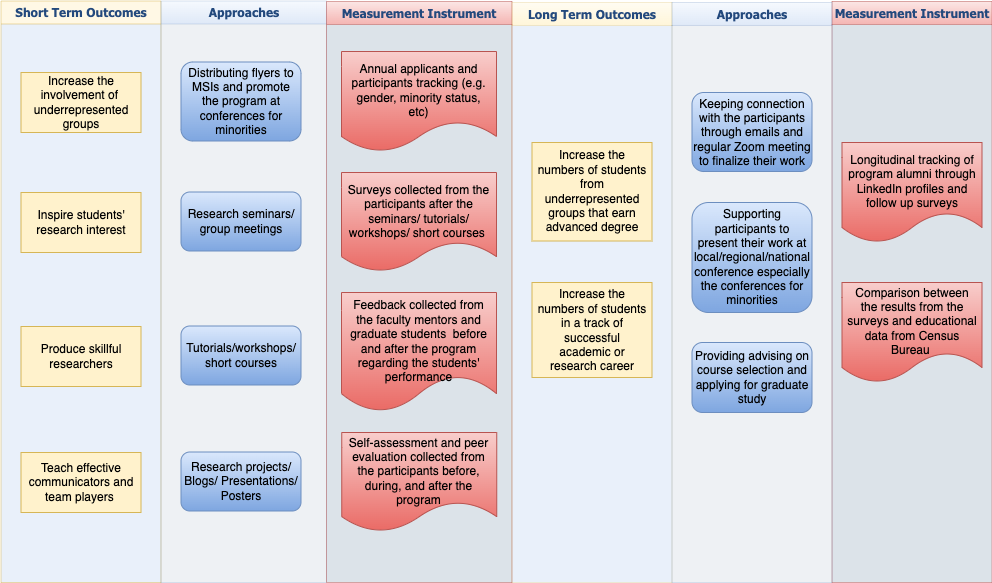
\includegraphics[width = 16cm]{EvalModel.png}
    \caption{Conceptual Model of the Evaluation}
    \label{fig:my_label}
\end{figure}

\subsection{Evaluation of Short Term Outcomes}

We will use survey form, feedback, and document review to evaluate the short-term outcomes. 
\GP and faculty mentors will develop the questionnaire that comprises these instruments to address the objectives. 

\subsubsection{Increase the Involvement of Underrepresented Groups}
We will track the demographic information of the applicants and participants. We expect that at least 20\% of the applicants will be from underrepresented groups. If we can't meet the targeted rate, we will spend more effort in connecting with more \MSIs and research-limited institutions and advertising SURE next year.  The annual report will document all the numbers, suggestions, and new strategies. 

\subsubsection{
Inspire Students' Research Interests to Explore Real-world Problems}

SURE participants will fill out a survey regarding the program's influence at the end of the program. They will be asked about the gain from the program, any changes in their future education and career plans after the program, and suggestions for the program. \GP will compare the acquired information with the motivation and career plans in the application materials. The result will provide the short-term influence of the SURE program on their career path.


\subsubsection{Produce Skillful Researchers} \label{sec:hardskill}
The research capability will be measured in four parts: learning new algorithms, identifying the problem, formulating the problem, and identifying the approaches.
Students will be asked to assess themselves within a range of 0 to 10 before and after the program. Faculty mentors will use the same survey to evaluate the student's research capability after the first two-week program and re-assess the students’ capability after the program based on their performance in the project.
The results of these assessments will provide a way to measure the improvement of the student's knowledge skills and research capabilities. Based on the analyses of the results, the faculty mentors will adjust the topics and designs of the courses, tutorials,  and workshops to enhance the training in the specific areas in the next year's program.
We will also collect feedback from the students after tutorials/workshops/seminars/short courses. This feedback will provide more direct ideas on organizing these activities efficiently.

\subsubsection{Teach Effective Communicators and Team Players}

``Soft'' skills, such as communication and teamwork, will be assessed by the participants and their team members before and after the program. In addition, the assessment will be collected from the faculty mentors and corresponding graduate students at the end of the second week and after the program. The same methodology as in Section \ref{sec:hardskill} will be implemented here. 




\subsection{Evaluation of Long Term Outcomes}

SURE participants will be encouraged to create LinkedIn profiles to catch up quickly in the future. They will complete follow-up surveys via email or during communication with their mentors. \GP will collect the percentage in advanced degrees of SURE alumni and SURE underrepresented alumni. The results will be compared with educational attainment data from Census Bureau. Based on the comparison outcome, \GP will propose the strategies to make the SURE program have more impact on participants’ education and career decisions. The annual report will document all numbers, results, and strategies.

\subsection{Evaluation of Implementation of the Program}
\GP will access all application materials and selection rubric after the students are selected. \GP will review materials, compare the students chosen to the established rubric, and verify that the rubric criterion has been followed. For comparison purposes, \GP will also
review the applicants who were not selected. Identified deviations will be immediately drawn to the attention of the selection committee. The most effective recruitment methods will be expanded in the following years, while the less effective ways will be redesigned or removed. Schedules, participation logs, possible research projects, and peer-reviewed papers will be maintained and provided to \GP. These documents will be reviewed to determine whether the program was implemented in the manner as it was proposed.

 
\section{Intellectual Merit}
The intellectual merit of the proposed work consists of (1) development of new computational finance methods to address financial crisis based on ESG scores; (2)
new and efficient methods in Monte Carlo sampling and development of corresponding algorithms and software based on these methods; (3) development of new energetic variational inference approach for machine learning ; (4) 
implement RQMC and the least square regression in pricing American options and comparison with other variance reduction methods; (5) development of a model in controlling nonlinear interface instability in Hele-Shaw flows and identifying critical physical parameters (critical evolution time and interface size) via a machine learning approach to achieve a dynamical equilibrium state and potential applications in physics and biology.
The proposed research will build on current results and contribute to new mathematical, statistical,
and computational methods, algorithm design, analysis, data collection, and implementation to address
important and complex problems in real life. New codes or algorithms will be made publicly
available on the program’s website and some open scholarships.

\section{Broader Impacts}
\begin{sloppypar}\Upara{Providing Research Experiences for Undergraduate} 
%%%%%%%%%%%%%%%%%%%%%%%%%%%%%%%%%%%%%%%%%%%%%%%%%%%%
SURE will promote advanced training in STEM
disciplines. The student-centered learning-researching modules will enhance participants’ knowledge in
mathematics and statistics and develop their capabilities in conducting independent research. This program will make a deliberate effort to diverse research environments by targeting female and underrepresented minority students as well as students from less research-focused institutions. \end{sloppypar}

%%%%%%%%%%%%%%%%%%%%%%%%%%%%%%%%%%%%%%%%%%%%%%%%%%%%
\Upara{Disseminating Research and Poster Presentation at Conferences}
%%%%%%%%%%%%%%%%%%%%%%%%%%%%%%%%%%%%%%%%%%%%%%%%%%%%
The research in SURE will result in publications in peer-reviewed journals in applied mathematics, computer science, statistics, and machine learning. These journals will include both those that emphasize theory and those that emphasize applications. \MAA Horizons is also a good candidate to submit the paper. All Illinois Tech SURE groups will be required to make posters and strongly encouraged to attend Illinois Tech research poster day in August. They will also join some local/regional/national conferences such as \MAA MathFest, \JMM, and \SIAM annual meeting, etc, to present the results of their work either in poster or presentation.


%%%%%%%%%%%%%%%%%%%%%%%%%%%%%%%%%%%%%%%%%%%%%%%%%%%%
\Upara{Preparing Students for Professional  Development} 
%%%%%%%%%%%%%%%%%%%%%%%%%%%%%%%%%%%%%%%%%%%%%%%%%%%%
SURE is committed to promoting research in computational mathematics and statistics and motivating undergraduates to pursue graduate careers in STEM disciplines and will also help current students land competitive jobs in the business world. Our training in the areas of computation and software development gives our students the needed edge in comparison to other mathematics graduates. SURE participants from different institutions through a series of educational and social activities will enhance their professional development and begin to form a network of partners with similar intellectual interests and goals. 

%%%%%%%%%%%%%%%%%%%%%%%%%%%%%%%%%%%%%%%%%%%%%%%%%%%%
\Upara{Community Impact}
%%%%%%%%%%%%%%%%%%%%%%%%%%%%%%%%%%%%%%%%%%%%%%%%%%%%
Illinois Tech is committed to serve working-class people. 
It has been ranked \#1 in Illinois and \#32 in the nation for lifting students from families in the bottom 20\% of income to the top 20\% \cite{IITrank}. 
The faculty and administration of Illinois Tech have been creating many innovative programs to achieve, such as the experiential learning opportunities offered by the existing Elevate Program \cite{IITElevate}.
The proposed SURE program is different from the existing programs since it is more research oriented whereas some other existing programs are more knowledge-learning oriented. 
We believe the proposed SURE program will fill a gap in training the research capabilities and enhance the broader impacts of Illinois Tech on its neighboring communities. 



%%%%%%%%%%%%%%%%%%%%%%%%%%%%%%%%%%%%%%%%%%%%%%%%%%%%
\Upara{Improving Illinois Tech}
%%%%%%%%%%%%%%%%%%%%%%%%%%%%%%%%%%%%%%%%%%%%%%%%%%%%
The Department of Applied Mathematics at Illinois Tech is committed to build a strong applied mathematics program with computational mathematics and data science as a major research area. 
SURE will generate more momentum and stimuli for our teaching and research in this area. We will attract more underrepresented undergraduate students to this research area. Through the SURE and the teaching and research materials/outcomes, we can add new components on computational mathematics and data science to the existing courses Math 478 Computational Mathematics, Math 569 Statistical Learning, Math 565 Monte Carlo Methods in Finance, and others.
We expect that students will establish a lasting interest in research in the interdisciplinary areas of mathematics and data science.



\section{Results from Prior NSF Support} \label{sec:prior_work}

\subsection{Yuhan Ding Has No Prior NSF Support}

\subsection{NSF-DMS-1522687, \emph{Stable, Efficient, Adaptive Algorithms for
			Approximation and Integration},
		\$270,000, August 2015 -- July 2018} \label{sec:PreviousFred}
%%%%%%%%%%%%%%%%%%%%%%%%%%%%%%%%%%%%%%%%%%%%%%%%%%%%%%%%%%%%%%%%%%%%%%%%%%%%%%%%%%%
Fred Hickernell (\FH, PI) and Gregory E. Fasshauer (\GEF, co-PI) led this project, and Sou-Cheng Choi (\SCTC) contributed as senior personnel.  Other contributors were \FH's research students {\YD} ( PhD 2015), \hypertarget{LJlink}{ Lan Jiang } (\LJ, PhD 2016),
\hypertarget{LlAJRlink}{Llu\'is Antoni Jim\'enez Rugama} (\LlAJR, PhD 2016), \hypertarget{DLlink}{Da Li} (\DL, MS 2016), \hypertarget{JLlink}{Jiazhen Liu} (\JL, MS 2018), JR (PhD 2019), \hypertarget{XTlink}{Xin Tong} (\XT, MS 2014, PhD 2020 at the University of Illinois at Chicago), \hypertarget{KZlink}{Kan Zhang} (\KZ, PhD student), \hypertarget{YZlink}{Yizhi Zhang} (\YZ, PhD 2018), and \hypertarget{XZlink}{Xuan Zhou} (\XZ, PhD 2015).  Articles, theses,
software, and preprints supported in
part by this
grant
include
\cite{ala_augmented_2017,
	ChoEtal17a,
	ChoEtal21a,
	Din15a,
	DinHic20a,
	GilEtal16a,
	Hic17a,
	HicJag18b,
	HicJim16a,
	HicEtal18a,
	HicEtal17a,
	HicKriWoz19a,
	RatHic19a,
	GilJim16b,
	JimHic16a,
	JohFasHic18a,
	Li16a,
	Liu17a,
	MarEtal18a,
	mccourt_stable_2017,
	MCCEtal19a,
	mishra_hybrid_2018,
	MisEtal19a,
	rashidinia_stable_2016,
	rashidinia_stable_2018,
	Zha18a,
	Zha17a,
	Zho15a,
	ZhoHic15a}.

%%%%%%%%%%%%%%%%%%%%%%%%%%%%%%%%%%%%%%%%%%%%%%%%%%%%%%%%%%%%%%%%%%%%%%%%%%%%%%%%%%%
\subsubsection{Intellectual Merit from Prior NSF Support}
\label{previousmeritsubsec}
%%%%%%%%%%%%%%%%%%%%%%%%%%%%%%%%%%%%%%%%%%%%%%%%%%%%%%%%%%%%%%%%%%%%%%%%%%%%%%%%%%%

\iffalse
\begin{wrapfigure}{r}{0.4\textwidth}
	\centering
	\vspace{-1ex}
	\includegraphics[width = 0.4\textwidth]{ProgramsImages/sampling-funappxg.png}
	\\
	\includegraphics[width = 0.4\textwidth]{ProgramsImages/sampling-funming.png}

	\vspace{-2ex}
	\caption{The function data ({\color{MATLABOrange}$\bullet$}) for the locally adaptive
		function approximation (top) and minimization (bottom) algorithms in \cite{ChoEtal17a}.  Sampling is denser where $\abs{f''}$ is larger.  For minimization it is also denser where the function values are smaller. \label{localadaptfig}}
\end{wrapfigure}
\fi

\FH, \SCTC, \YD, \XT, \YZ developed several adaptive algorithms for univariate integration, function approximation, and optimization \cite{ChoEtal17a,HicEtal14b,  Din15a, Ton14a, Zha18a}.  Those constructed by \FH, \SCTC, \YD, and \XT in \cite{ChoEtal17a} are \emph{locally adaptive}---the nonuniform sampling density is influenced by the function data.  For function approximation, the computational cost of $\Order\left(\sqrt{\norm[1/2]{f''}/\varepsilon} \right)$, where $\varepsilon$ is the error tolerance, and is essentially optimal. 
\FH, \LlAJR, \DL, and \JR developed globally adaptive algorithms for approximating $\int_{[0,1]^d} f(\bx) \, \dif \bx$ based on LD sequences \cite{HicJim16a,HicEtal17a,JimHic16a}. 
\FH, \YD, \LlAJR, and collaborators investigated function approximation problems for Banach spaces, $\calf$, defined by series representations \cite{DinHic20a,DinEtal20a}.  Adaptive function approximation algorithms constructed were shown to be essentially optimal.


%%%%%%%%%%%%%%%%%%%%%%%%%%%%%%%%%%%%%%%%%%%%%%%%%%%%%%%%%%%%%%%%%%%%%%%%%%%%%%%%%%%
\subsubsection{Broader Impacts from Prior NSF Support} \label{prevBIsect}
%%%%%%%%%%%%%%%%%%%%%%%%%%%%%%%%%%%%%%%%%%%%%%%%%%%%%%%%%%%%%%%%%%%%%%%%%%%%%%%%%%%
Publications by \GEF, \FH,  \SCTC, students, and collaborators are listed above.  We have spoken at many applied mathematics, statistics,
and computational science conferences and given colloquium/seminar talks to mathematics and
statistics departments.  \FH co-organized the
2016 Spring Research
Conference, \FH gave an invited tutorial
at MCQMC 2016
\cite{Hic17a}, was a program leader for the SAMSI 2017--18 Quasi-Monte Carlo (QMC) Program, and received the 2016 Joseph F.\ Traub Prize for Achievement in Information-Based Complexity.  This research has been implemented in our open-source library
\GAIL \cite{ChoEtal21a}.  \SCTC has been key in this effort.  \GAIL has been used in the graduate Monte Carlo course taught by \FH and \YD. \GEF, \FH, and \SCTC mentored a number of
research students;  female students include \YD, \LJ, \JL, \XT, and Xiaoyang Zhao (MS 2017).

%{\bf Kang} serves as the PI for ``Statistical Design, Sampling, and Analysis for Large Scale Experiments'' (DMS-1916467, \$ 120,000, 09/2019–08/2022). {\bf Intellectual Merits:} The project covers topics in statistical design theories and algorithms for various types of experiments, active learning,195 and Bayesian modeling for mixed outcomes data.196 These works have provided significant insights into the optimal design theories, efficient and theoretically-sound design and active learning algorithms, new statistical sampling approaches, and new statistical modeling approach for complex data. Kang also created a particle-based energetic variational inference approach.197 {\bf Broader Impacts:} The research results have provided fundamental insights into chemical and materials sciences by applying active learning approaches. The research products have been disseminated through publications, conferences, and workshops and are available through public repositories (arXiv and GitHub). New course modules were developed for graduate students. One PhD student is currently being supported by this grant. 

%[LK1] Y. Li, L. Kang, and X. Deng, (2021) A Maximin Phi_p-Efficient Design for Multivariate GLM. arXiv preprint arXiv:2008.06475
%[LK2]Q. Zhang, and L. Kang, (2020) Optimal Design for A/B Testing in the Presence of Covariates and Network Connection. 1–27, 2020. arXiv preprint arXiv:2008.06476
%[LK3] Y. Li, L. Kang, and X. Huang, (2021) Covariate Balancing Based on Kernel Density Estimates for Controlled Experiments. Statistical Theory and Related Fields. DOI: 10.1080/24754269.2021.1878742.
%[LK4] Chen, J., Kang, L., and Lin, G. (2020) Gaussian Process Assisted Active Learning of Physical Laws. Technometrics. DOI: 10.1080/00401706.2020.1817790
%[LK5]	Kang, X., Ranganathan, S., Kang, L., Gohlke, J., Deng, X. (2020) Bayesian Quantitative- Qualitative Model via Latent Variable with Application to Birth Records Data. arXiv preprint arXiv:2008.06525.
%[LK6]	Wang, Y., Chen, J., Liu, C., and Kang, L. (2020) Particle-Based Energetic Variational Inference. arXiv preprint arXiv:2004.06443


\newpage
\clearpage
\setcounter{page}{1}

\pagestyle{empty} %to eliminate page numbers for upload
%\pagestyle{plain} %to add back page numbers

\bibliographystyle{spbasic.bst} 

\renewcommand{\refname}{{\Large\textbf{References Cited}}} %%
 
%\scnote{Some journals are abbreviated (e.g., J Complexity), while others are not (e.g., Journal of the American Statistical Association).}

\renewcommand{\bibliofont}{\normalsize}

\bibliography{FJH23,FJHown23,EVI,kang,sc,Li,Ding}
\end{document}


%%%%%%%%%%%%%%%%%%%%%%%%%%%%%%%%%%%%%%%%%%%%%%%%%%%%
\Upara{Recruitment and Application Materials} 
%%%%%%%%%%%%%%%%%%%%%%%%%%%%%%%%%%%%%%%%%%%%%%%%%%%%
All recruitment and application materials will be shared
with \GP before and after implementation, including the applicant selection rubric. \GP will review
the application materials and the selection rubric, and provide formative feedback to faculty mentors
before the materials are distributed and before students are selected. After the students are selected
but before they are formally accepted, \GP will compare the selected students to the established
rubric and verify that the rubric criterion has been followed. For comparison purposes, \GP will also
review the applicants who were not selected. Identified deviations will be immediately drawn to the
attention of the selection committee. The most effective recruitment methods will be expanded in the
years that follow while the less effective methods will be redesigned or removed. \GP will review the
recruitment process and results of the process for summative purposes. Baseline data will be collected
concerning students’ prior mathematics and statistics courses, computer skills, and research experiences.


%%%%%%%%%%%%%%%%%%%%%%%%%%%%%%%%%%%%%%%%%%%%%%%%%%%%
\Upara{Survey Forms} 
%%%%%%%%%%%%%%%%%%%%%%%%%%%%%%%%%%%%%%%%%%%%%%%%%%%%
Surveys will be administered to SURE participants and faculty mentors before, during, and after the program. The questions that comprise these instruments will be developed under the leadership of the evaluator and faculty mentors to address the objectives.
Students will be asked to assess their research capability in identifying the problem, formulating the problem, identifying the approaches,  learning new algorithms, and communicating with others before and after the program.
Faculty mentors will use the same survey to evaluate the students' research capability after the first two-week program. Faculty mentors will re-assess the students' capability based on their performance in the project after the program.
The feedback of these two assessments will provide a way to measure the development of the students' knowledge skills and research capabilities in mathematics and statistics. If the development in some areas is quite limited, we will adjust the design of the workshops and tutorials to enhance the training in the specific areas in next year's program.
In addition, SURE participants' intention to pursue a research career will be collected in the survey before and after the program. Participants' response on how does SURE affect their career choice will also be collected. 
SURE participants will also be asked to complete follow-up surveys via email or communication with their mentors, concerning a longer-term program impact on their education and
career decisions. All this information will be used to track SURE participants into their careers aiming
to gauge the degree to which the program has been a lasting influence on SURE students’ career paths.

%%%%%%%%%%%%%%%%%%%%%%%%%%%%%%%%%%%%%%%%%%%%%%%%%%%%
\Upara{Document Review} 
%%%%%%%%%%%%%%%%%%%%%%%%%%%%%%%%%%%%%%%%%%%%%%%%%%%%
Application materials,  schedules,  possible research projects, and peer-reviewed papers will be maintained and provided
to \GP. These documents will be reviewed to determine whether the program was implemented
in the manner that it was proposed. Information acquired will be used to improve this
program. The papers co-authored by SURE participants will be used for summative evaluation, including
their development in knowledge and research skills. Application materials will also be examined to
determine whether SURE participants who successfully published peer-reviewed papers had entered this
program with different background knowledge or experiences than those that did not.
In addition, we will track the percentage of our targeted group of applicants and participants. If in some groups, the percentage is quite low, we will spend more effort on advising our program in that group. The annual report will also address whether we reach the targeted percentage or not. If not, \GP will suggest several ways to be conducted in the next year.
